% VIGTIGT! For at dokumentet kan kompilere, skal man benytte XeLaTeX eller LuaLaTeX som compiler. Dette kan gøres i Overleaf ved at gå til Menu -> Settings -> Compiler -> Vælg XeLaTeX/LuaLaTeX
\documentclass[10pt,a4paper,twoside]{article}

\usepackage[numbers]{natbib} % Referencehåndtering til referencer.bib
\usepackage{KUstyle}
\usepackage[a4paper,inner=2.8cm,outer=3.2cm,top=3.5cm,bottom=3cm]{geometry} % Pakke til sidemargin
\usepackage{setspace} % Pakke til halvanden linjeafstand
\usepackage{tabularx} % Pakke til tabel
\usepackage{fontspec}
\usepackage[danish]{babel}
\usepackage{microtype}
\usepackage{pdflscape}
\usepackage{caption}
\captionsetup{hypcap=false,font=small,labelfont=bf,justification=raggedright,singlelinecheck=false}
\usepackage{tikz}
\usetikzlibrary{arrows.meta,shapes.geometric}

\IfFontExistsTF{Linux Libertine O}
  {\setmainfont{Linux Libertine O}}
  {\IfFontExistsTF{Libertinus Serif}
    {\setmainfont{Libertinus Serif}}
    {\IfFontExistsTF{Times New Roman}
      {\setmainfont{Times New Roman}}
      {\IfFontExistsTF{Georgia}{\setmainfont{Georgia}}{\setmainfont{Times}}}}}
\setsansfont{Arial}
\setlength{\emergencystretch}{3em}
\setlength{\parindent}{0pt}
\setlength{\parskip}{1ex plus 0.5ex minus 0.2ex}
\setcounter{tocdepth}{2}
\setcounter{secnumdepth}{2}
\tolerance=9999
\hyphenpenalty=10000
\exhyphenpenalty=100

% Nedenstående ændrer indholdet på forsiden
\kuheaderone{KØBENHAVNS UNIVERSITET}
\kuheadertwo{DET SUNDHEDSVIDENSKABELIGE FAKULTET}
\kucoverbackground{assets/ku-cover-background-blue.png}
\kuheadercolor{black}
\kuheaderbackgroundwidth{120mm}
\kudegree{Bachelor i Sundhed og Informatik}
\kuunit{Institut for Folkesundhedsvidenskab}
\kudepartment{Afdeling for Sundhedstjenesteforskning}
\ptype{Bachelorprojekt}
\author{Christian Kristensen, TDH522}
\title{Træningsmester}
\subtitle{Design og implementering af en digital træningsapp til fleksibel progression og motivation}
\date{Afventer}
\advisor{Karsten Vrangbæk}
\fpimage{assets/traeningsmester-logo-uden-baggrund.pdf} % Kilde-SVG ligger i assets/traeningsmester-logo-uden-baggrund.svg

\renewcommand{\contentsname}{Indhold}
\addto\captionsdanish{\renewcommand{\contentsname}{Indhold}}
\renewcommand{\refname}{Referencer}
\renewcommand{\figurename}{Figur}
\renewcommand{\tablename}{Tabel}

\makeatletter
\newif\iftmappendix
\tmappendixfalse
\let\tmoldappendix\appendix
\renewcommand{\appendix}{\tmoldappendix\tmappendixtrue}

\newcommand{\tmheadinglabel}[1]{%
  \iftmappendix
    \MakeUppercase{Bilag}~#1%
  \else
    \MakeUppercase{Kapitel}~#1%
  \fi
}

\newcommand{\tmchapterheading}[2]{%
  \clearpage
  \thispagestyle{plain}%
  \begingroup
  \setlength{\parskip}{0pt}%
  \vspace*{0.8cm}%
  \noindent\hfill{\normalfont\normalsize\tmheadinglabel{#1}}\par
  \vspace{0.8ex}%
  \noindent\rule{\textwidth}{0.4pt}\par
  \vspace{0.45ex}%
  \noindent\hfill{\normalfont\normalsize\bfseries #2}\par
  \vspace{0.45ex}%
  \noindent\rule{\textwidth}{0.4pt}\par
  \endgroup
  \vspace{0.85cm}%
}

\newcommand{\tmplainheading}[1]{%
  \clearpage
  \thispagestyle{plain}%
  \begingroup
  \setlength{\parskip}{0pt}%
  \vspace*{1.4cm}%
  \noindent\rule{\textwidth}{0.4pt}\par
  \vspace{0.45ex}%
  \noindent\hfill{\normalfont\normalsize\bfseries #1}\par
  \vspace{0.45ex}%
  \noindent\rule{\textwidth}{0.4pt}\par
  \endgroup
  \vspace{0.85cm}%
}

\renewcommand\section{%
  \@ifstar{\tmsectionstar}{\tmsectionnumbered}%
}
\newcommand{\tmsectionnumbered}[1]{%
  \refstepcounter{section}%
  \addcontentsline{toc}{section}{\protect\numberline{\thesection}#1}%
  \tmchapterheading{\thesection}{#1}%
}
\newcommand{\tmsectionstar}[1]{%
  \tmplainheading{#1}%
}

\renewcommand\subsection{\@startsection{subsection}{2}{\z@}%
  {-2.2ex plus -1ex minus -.2ex}%
  {0.9ex plus .2ex}%
  {\normalfont\normalsize\bfseries\raggedright}}
\renewcommand\subsubsection{\@startsection{subsubsection}{3}{\z@}%
  {-1.8ex plus -0.8ex minus -.2ex}%
  {0.7ex plus .2ex}%
  {\normalfont\normalsize\bfseries\raggedright}}

\renewcommand\tableofcontents{%
  \tmplainheading{\contentsname}%
  \@starttoc{toc}%
}
\makeatother

\begin{document}

\pagenumbering{gobble}
\makeprojecttitle
\makekutitle

\setstretch{1}

\pagenumbering{roman}
\setcounter{page}{1}
\begin{table}[h]
\def\arraystretch{1.5}
\begin{tabularx}{\textwidth}{l >{\raggedright\arraybackslash}X}
Fakultet: & Det Sundhedsvidenskabelige Fakultet \\
Institutnavn: & Institut for Folkesundhedsvidenskab \\
Afdelingsnavn: & Afdeling for Sundhedstjenesteforskning \\
Uddannelse: & Bachelor i Sundhed og Informatik \\
Forfatter(e): & Christian Kristensen, TDH522 \\
Titel og evt. undertitel: & Træningsmester: Design og implementering af en digital træningsapp til fleksibel progression og motivation \\
Emnebeskrivelse: & Projektet undersøger, hvordan en digital træningsapp kan designes og implementeres, så programstruktur, progression og feedback understøtter vedvarende motivation og fleksibel håndtering af afvigelser fra et planlagt træningsforløb uden at øge risikoen for demotivation og frafald. \\
Vejleder: & Karsten Vrangbæk \\
Dato: & Afventer
\end{tabularx}
\end{table}
\newpage

\phantomsection
\addcontentsline{toc}{section}{\contentsname}
\tableofcontents
\newpage

\pagenumbering{arabic}
\setcounter{page}{1}

\section{Indledning}

\emph{Digitale træningsapps} kan gøre træningsprogrammer, øvelser, historik og feedback lettere tilgængelige. Det løser dog kun en del af problemet. Vedvarende fysisk aktivitet hænger også sammen med autonom motivation, oplevet kompetence og støtte, der giver brugeren en meningsfuld oplevelse af kontrol \cite{teixeira2012_sdt_exercise}. Digital brug har først værdi, når den faktisk støtter den ønskede adfærd og ikke blot skaber mere skærmtid \cite{yardley2016_effective_engagement_dbci}.

I praksis møder træningsplanen en hverdag med begrænset tid, ændret dagsform, fyldt træningscenter, skiftede øvelser og ufuldstændig \emph{logging}. Den slags besvær betegnes som \emph{friktion}. Hvis appen kun giver mening ved perfekt efterlevelse, bliver støtten svag netop i de situationer, hvor brugeren har mest brug for overblik.

Den afgørende forskel ligger mellem en plan, der ser rigtig ud på forhånd, og et forløb, der stadig giver mening bagefter. En kalender kan fortælle, hvad brugeren skulle have gjort. En brugbar træningsapp skal også kunne håndtere, hvad brugeren faktisk gjorde, og omsætte det til en næste handling uden at gøre ændringen til et nederlag.

Apps og aktivitetsmålere kan understøtte fysisk aktivitet, men studierne peger samtidig på, at effekten varierer med design, brugskontekst og vedvarende anvendelse \cite{laranjo2021_apps_trackers_meta,romeo2019_smartphone_apps_pa_meta,brickwood2019_wearable_trackers_meta}. Frafald er derfor et centralt vilkår i digitale sundhedsinterventioner. Når brugeren stopper, før interventionen kan få virkning, mister løsningen sin praktiske værdi \cite{eysenbach2005_law_of_attrition}.

I styrketræning bliver udfordringen mere konkret, fordi et program rummer mere end en kalender. American College of Sports Medicine (ACSM) beskriver progression gennem belastning, volumen, øvelsesvalg, frekvens og løbende justering \cite{acsm2009_progression_models}. Nyere resistance-training-anbefalinger fastholder progression som et centralt princip, mens forskning i autoregulering gør justering efter dagsform og performance fagligt relevant \cite{currier2026_acsm_resistance_training,greig2020_autoregulation_resistance_training,larsen2021_autoregulation_systematic_review}.

TræningsMester er udviklet som en \emph{native iOS-app}, hvor denne spænding bliver konkret. Plan, tracker, completion, feedback og næste handling mødes i samme brugerforløb. Brugeren kan springe et pas over, ændre belastning, bytte øvelser, træne uden at logge alle sæt eller vende tilbage efter en afbrudt session. Appens centrale udfordring er at fastholde retning og progression, når træningen ikke følger en perfekt lineær plan.

\tmdelkonklusion{Mellempointe}{Problemet er bruddet mellem plan og hverdag. En brugbar træningsapp skal kunne vise, at brugeren stadig er i gang, og hvad næste skridt er, også når træningen ikke blev logget perfekt.}


\section{Problemformulering og afgrænsning}

\subsection{Problemformulering}

Problemet ligger i krydsfeltet mellem fysisk aktivitet, digital adfærdsstøtte, interaktionsdesign og softwareudvikling. Motivation, engagement og frafald er centrale i digitale sundhedsinterventioner, mens styrketræning kræver en model for progression, justering og realistiske ændringer i planen \cite{teixeira2012_sdt_exercise,eysenbach2005_law_of_attrition,acsm2009_progression_models}. Hovedspørgsmålet er:

\begin{quote}
Hvordan kan en digital træningsapp designes og implementeres, så programstruktur, progression og feedback understøtter vedvarende motivation og fleksibel håndtering af afvigelser fra et planlagt træningsforløb uden at øge risikoen for demotivation og frafald?
\end{quote}

Spørgsmålet styrer en design- og implementeringsundersøgelse. TræningsMester vurderes som en udviklet app, hvor struktur, feedback, brugsmæssigt besvær og sikker dataadgang skal hænge sammen. Evidensniveauet er derfor knyttet til appens design, implementering, dokumenterede artefakter og tekniske verifikation.

Appen placeres på det første nødvendige trin før en senere effektmåling. Før man kan undersøge, om en intervention ændrer fysisk aktivitet eller fastholdelse i en brugerpopulation, skal træningsmodel, brugerflows, feedback, datamodel og adgangsregler kunne beskrives og vurderes samlet.

\subsection{Underspørgsmål}

Hovedspørgsmålet konkretiseres i fire underspørgsmål:

\begin{enumerate}
    \item Hvordan kan plan, \emph{workout}, \emph{trackerlog}, \emph{completion-event} og \emph{cycle runtime} modelleres, så faktisk træning kan afvige fra planen uden datatab?
    \item Hvordan kan brugerfladen reducere friktion under træning, herunder \emph{tracker-off flow}, \emph{watchOS} og \emph{Live Activity}?
    \item Hvordan kan \emph{Supabase}, \emph{Row Level Security} (RLS), \emph{repositories} og \emph{Edge Functions} understøtte fleksible brugerflows uden privilegeret adgang i klienten?
    \item Hvordan kan \emph{beta-feedback}, skærmbilleder, \emph{build}- og testresultater samt diagrammer bruges som evidens for design- og implementeringsvalg?
\end{enumerate}

De fire spørgsmål følger den faglige afhængighed mellem model, brugssituation, adgangskontrol og evidens. Først skal træningen modelleres, så plan og faktisk udførelse ikke blandes sammen. Dernæst skal modellen kunne bruges i en travl træningssituation. Derefter skal dataadgangen afgrænses, så fleksibilitet bygger på kontrollerede rettigheder. Til sidst skal belægget vurderes nøgternt, så dokumenteret systemdesign, kvalitativ brugerindsigt og senere effektstudier ikke blandes sammen.

\subsection{Egenudviklet app og afgrænsning}

TræningsMester er en egenudviklet træningsapp og fungerer som \emph{design- og implementeringscase}. Appen samler planlagt programstruktur, tracker, completion, Home-flow, watchOS, Live Activity, datamodel og backendregler i ét system. Use cases, krav og tracker/completion-diagram kobler brugerhandlinger med krav, implementeringsspor og progression.

SwiftUI, Supabase, RLS, Edge Functions, watchOS og Live Activity indgår som dele af den udviklede løsning. De er relevante, når de håndterer ændringer i træningsforløbet, reducerer betjeningsbesvær eller beskytter brugerdata.

Afgrænsningen har fire praktiske konsekvenser. Appens sundhedseffekt hører til et senere effektstudie. Abonnement, admin, import og trænerfunktioner indgår som støttefunktioner, når de belyser progression, datakvalitet eller sikkerhed. Sikkerhed vurderes som design, arkitektur og delvis verifikation med GDPR, OWASP MASVS og Supabase RLS som rammer \cite{europeanparliament2016_gdpr,owasp2024_masvs,supabase_rls_docs}. HealthKit og platformintegrationer behandles som fitnessnære appintegrationer, mens klinisk journaludveksling hører uden for den udviklede løsning.

\subsection{Faglig model}

TræningsMesters centrale model adskiller planlagt træning, faktisk logging, completion og næste handling. En almindelig logbog gemmer fortiden. TræningsMester bruger også fortiden til at gøre næste træningsvalg forståeligt. Den adskillelse kan bevare historik og progression, selv når brugeren ikke følger en perfekt lineær plan.

\tmdelkonklusion{Kernevalg}{Kernen i TræningsMester er spændingen mellem struktur og ændringer i praksis. Appen står stærkest, når plan, handling og data hænger sammen. De stærkeste påstande handler derfor om dokumenteret design og implementering frem for effekt uden et egentligt effektstudie.}


\section{Teoretisk og faglig ramme}

TræningsMester vurderes ud fra fire faglige spor. Det første spor handler om motivation, frafald og effektivt engagement. Det andet handler om app- og tracker-evidens samt appkvalitet. Det tredje handler om progression og autoregulering i styrketræning. Det fjerde handler om interaktionsdesign, datakvalitet og sikkerhed. Tilsammen afgør sporene, om appen kan forbinde plan, faktisk træning, feedback og dataansvar i samme system.

\subsection{Motivation, frafald og effektivt engagement}

Vedvarende fysisk aktivitet er tæt knyttet til autonom motivation, oplevet kompetence og støtte, der giver brugeren meningsfuld kontrol \cite{teixeira2012_sdt_exercise}. For en træningsapp betyder det, at feedback skal hjælpe brugeren videre frem for kun at markere, om en plan blev fulgt korrekt.

Frafald er et grundvilkår i digitale sundhedsinterventioner, fordi mange brugere stopper, før interventionen kan få virkning \cite{eysenbach2005_law_of_attrition}. Derfor bliver appens håndtering af ændringer i planen relevant. Hvis en afbrudt session eller manglende detaljelog opleves som et nederlag, kan brugerens vej tilbage til træningen blive sværere.

Effektivt digitalt engagement handler om brug, der støtter den ønskede adfærd frem for blot mange klik eller meget data \cite{yardley2016_effective_engagement_dbci}. COM-B og Behaviour Change Technique Taxonomy giver et sprog for capability, opportunity, motivation, selvmonitorering, mål og feedback \cite{michie2011_behaviour_change_wheel,michie2013_bct_taxonomy_v1}. I TræningsMester bruges disse begreber til at vurdere, om brugeren får en næste handling, der stadig føles legitim efter ændringer i træningen.

\subsection{Apps, trackers og appkvalitet}

Systematiske reviews og meta-analyser viser, at smartphoneapps og activity trackers kan øge fysisk aktivitet hos voksne, men effekterne varierer med intervention, målgruppe og brug \cite{laranjo2021_apps_trackers_meta,romeo2019_smartphone_apps_pa_meta}. Wearables kan også støtte fysisk aktivitet, især når feedback og mål er tydelige \cite{brickwood2019_wearable_trackers_meta}. Denne litteratur gør appsporet relevant for TræningsMester, samtidig med at appens effekt skal vurderes i senere bruger- og effektstudier.

Mobile App Rating Scale (MARS) gør appkvalitet til mere end funktionalitet. Engagement, informationskvalitet, æstetik og brugbarhed indgår også \cite{stoyanov2015_mobile_app_rating_scale}. Analyser af fysisk aktivitetsapps viser desuden, at mange apps kun delvist afspejler evidensinformerede adfærdsprincipper \cite{bondaronek2018_quality_pa_apps,kebede2018_evidence_informed_pa_apps,conroy2014_bct_top_ranked_pa_apps}. Derfor vurderes TræningsMester ikke på funktionsmængde, men på om funktionerne hænger sammen med progression, feedback og lavt betjeningsbesvær.

Litteraturen giver to kriterier for TræningsMester. Appen skal have en tydelig adfærdsfunktion, hvor selvmonitorering, mål, feedback og handlingsstøtte hænger sammen. Interaktionen skal samtidig være praktisk nok til, at brugeren kan bruge den under træning.

\subsection{Forskningsstatus og fagligt hul}

Eksisterende app- og trackerforskning giver et solidt grundlag for at se digital feedback og selvmonitorering som relevante for fysisk aktivitet. Meget af litteraturen handler dog om generel aktivitet, skridt, vægt eller brede mHealth-interventioner. Styrketræning kræver en mere detaljeret model for øvelser, sæt, belastning, progression og ændringer i den planlagte træning.

Det faglige hul ligger derfor i koblingen mellem adfærdsstøtte, programlogik, lavt betjeningsbesvær og sikker dataadgang i én styrketræningsapp. Hvis sporene behandles hver for sig, bliver løsningen enten en generel motivationsapp, en teknisk logbog eller en database med brugerflade. TræningsMester samler design og implementering omkring den praktiske test: om motivation, progression, data og adgang stadig hænger sammen, når brugeren træner anderledes end planlagt.

Den faglige værdi ligger i oversættelsen fra litteratur til app. TræningsMester skaber en konkret model for, hvordan kendte principper om motivation, feedback, progression, datakvalitet og adgangskontrol kan bygges ind i et system til realistisk træningsadfærd.

\subsection{Progression og autoregulering i styrketræning}

Styrketræning adskiller sig fra generel aktivitetsregistrering, fordi progression afhænger af øvelser, sæt, gentagelser, belastning, volumen, intensitet og restitution. ACSM beskriver, hvordan belastning, volumen, øvelsesvalg og frekvens reguleres over tid \cite{acsm2009_progression_models}. Nyere resistance-training-anbefalinger fastholder progression og tilpasning som centrale principper \cite{currier2026_acsm_resistance_training}.

Autoregulering gør det relevant at justere træning efter performance, readiness og dagsform \cite{greig2020_autoregulation_resistance_training,larsen2021_autoregulation_systematic_review}. En app bør derfor skelne mellem planlagt workout, faktisk trackerlog, completion-event og næste relevante træningshandling. Tracker/completion-diagrammet belyser denne adskillelse i TræningsMester.

ecofit-studiet viser, at mHealth kan indgå i en resistance-training-nær intervention \cite{plotnikoff2023_ecofit_rct}. Studiet fungerer som kontekstnær inspiration, mens vurderingen af TræningsMester bygger på design, implementering og verifikation.

Progression skaber også et datakrav. Appen skal kunne se forskel på en planlagt øvelse, en udført øvelse og en gennemført workout uden fulde detaljer. Samtidig kan et for detaljeret krav om logging gøre registreringen tung. Den faglige løsning er derfor ikke maksimal dataregistrering, men passende datagranularitet til formålet.

\subsection{Interaktionsdesign, datakvalitet og sikkerhed}

Interaktionsdesign handler om brugerens konkrete møde med systemet. Kursusgrundlaget om brugerundersøgelser, prototyper og evaluering peger på, at designvalg skal vurderes i den kontekst, hvor systemet bruges \cite{hornbaek2024_brugerundersoegelser,hornbaek2024_prototyper,hornbaek2024_evaluering}. I en træningssituation er brugerens opmærksomhed delt mellem krop, udstyr, omgivelser og app. Lav friktion betyder derfor lavt betjeningsbesvær frem for blot et pænt skærmlayout.

Datakvalitet skal vurderes efter formål og kontekst \cite{mohammed2025_five_facets_data_quality}. En trackerlog giver høj detaljeringsgrad, mens et completion-event kan bevare historik og næste handling, når brugeren ikke logger alle sæt. Data er dermed gode til forskellige formål, og appens model skal gøre forskellen tydelig.

Sikkerhed er en designbetingelse. OWASP MASVS beskriver principper for mobil datahåndtering og backendgrænser, mens Supabase RLS-dokumentationen viser, hvordan adgang kan begrænses efter bruger og rolle \cite{owasp2024_masvs,supabase_rls_docs,supabase_securing_api_docs}. GDPR fungerer som juridisk ramme for persondata \cite{europeanparliament2016_gdpr}. I TræningsMester bruges disse kilder til at vurdere adgangsmodellen. Bilagets sikkerhedsdiagram viser den centrale grænse mellem klient, RLS og Edge Functions, jf. Figur~\ref{fig:tm-security-boundary-summary}.

Rammen peger samlet på ét krav. Appen skal gøre den lette handling mulig og samtidig bevare en meningsfuld og sikker datamodel. Det er denne spænding mellem betjeningsbesvær, datakvalitet og adgangskontrol, der gør TræningsMester relevant for sundhedsinformatik.

\subsection{Operationalisering af rammen}

De faglige spor omsættes til fire vurderingsspørgsmål. Får brugeren en reel handlemulighed, når planen ændrer sig? Modelleres progression som mere end en kalender, så plan, faktisk logging, completion og næste handling kan adskilles? Kan brugerfladen bruges midt i træningen uden unødigt registreringsarbejde? Er datakvalitet og adgangskontrol stærke nok til at bære fleksible flows uden at gøre klienten til sikkerhedsautoritet?

\tmdelkonklusion{Teoriens konsekvens}{Et stærkt designvalg skal kunne forklares fagligt, ses i appen og afgrænses metodisk. Hvis et valg kun findes i litteraturen, er det en intention. Hvis det kun findes i koden, er det en funktion. Først når begge dele mødes, bliver valget fagligt relevant.}


\section{Metode}

TræningsMester behandles som en \emph{design- og implementeringscase}. Metoden kombinerer kildesøgning, kursus- og faggrundlag, \emph{artefaktanalyse}, anonymiseret beta-feedback og teknisk verifikation. Samlet kan materialet vurdere, om appens design og implementering hænger fagligt og teknisk sammen.

Metodevalget følger problemformuleringen. Spørgsmålet handler om, hvordan en app kan designes og implementeres, så programstruktur, progression og feedback understøtter fleksibel træning. Derfor vægtes dokumenterede designvalg, implementeringsspor, krav, tests og kvalitativ feedback højere end kvantitative effektmål.

\subsection{Design- og implementeringscase}

\emph{Caseformen} bruges om den egenudviklede app. Den gør det muligt at undersøge, hvordan teori om motivation, progression, friktion og sikker dataadgang omsættes til et konkret digitalt system. TræningsMester vurderes gennem synlige brugerflader, krav, arkitektur, datamodel og testspor. Bilagets materialegennemgang samler de synlige artefakter, og systemkontekstdiagrammet viser de centrale platforme og services, jf. Tabel~\ref{tab:tm-bilag-materialegennemgang} og Figur~\ref{fig:tm-system-context}.

Evidensniveauet er design- og implementeringsplausibilitet. Det betyder, at analysen kan vurdere sammenhængen mellem problem, løsning og dokumentation, mens bred brugeraccept og sundhedseffekt kræver senere undersøgelser.

Vurderingen følger en enkel kæde. Først fastlægges det faglige problem. Derefter omsættes problemet til krav og use cases. Til sidst vurderes arkitektur, implementering, test og feedback. Kæden er vigtig, fordi en pæn brugerflade ikke er nok alene, og en solid datamodel først får værdi, når brugeren kan komme gennem træningen med lavt betjeningsbesvær.

\subsection{Analysegenstand}

\emph{Analysegenstanden} er den udviklede apps håndtering af ændringer i et træningsforløb. Appen analyseres som en kæde af mekanismer med planlagt workout, aktiv tracker, completion-event, cycle runtime, næste handling, brugerfladefeedback og adgangskontrol.

Genstanden undersøges på tre niveauer. Det træningsfaglige niveau handler om, hvorvidt modellen kan bevare progression, når faktisk træning afviger fra planen. Interaktionsniveauet handler om, hvorvidt Home, tracker, tracker-off, watchOS og Live Activity kan reducere betjeningsbesvær i selve træningssituationen. Det informatiske niveau handler om, hvorvidt datamodel, RLS, repositories og Edge Functions gør fleksibiliteten sporbar og adgangsmæssigt afgrænset.

Denne afgrænsning gør analysen vurderbar. De centrale dele er dem, der afgør, om spændingen mellem struktur og ændringer i praksis kan håndteres.

\subsection{Analysestrategi}

Analysestrategien følger underspørgsmålene. Tabel~\ref{tab:analysestrategi} kobler materialetyper med vurderingskriterier og markerer grænsen mellem plausibilitet, brugerindsigt og effektbevis.

\begin{table}[h]
\small
\renewcommand{\arraystretch}{1.14}
\begin{tabularx}{\textwidth}{p{0.24\textwidth} Y Y}
\toprule
\tmthead{Underspørgsmål} & \tmthead{Materiale} & \tmthead{Vurderingskriterium} \\
\midrule
Plan, trackerlog, completion og cycle runtime & Use cases, kravsporbarhed, datamodel, trackerproces og implementeringsbeskrivelse & Om planlagt og faktisk træning kan adskilles uden datatab, og om næste handling kan forklares efter ændringer i forløbet. \\
\emph{UI} og lav friktion & Skærmbilleder, interaktionsdesign, beta-feedback og støtteflader for watchOS og Live Activity & Om brugeren får tydelig status, feedback og næste handling uden unødigt registreringsarbejde. \\
Sikker dataadgang & Sikkerhedsgrænse, RLS-matrix, Edge Function-spor og tekniske primærkilder & Om privilegeret logik holdes uden for klienten, og om påstande afgrænses til dokumenteret design og delvis test. \\
Evidensgrundlag & Kildesøgning, anonymiseret feedback, build- og testspor, skærmbilleder og diagrammer & Om dokumenterede artefakter tydeligt skelner mellem plausibilitet, brugerindsigt og effektbevis. \\
\bottomrule
\end{tabularx}
\caption{Analysestrategi for koblingen mellem underspørgsmål, materiale og vurderingskriterier.}
\label{tab:analysestrategi}
\end{table}

Et stærkt belæg kræver mere end mange bilag. Teori, krav, implementering og verifikation skal pege i samme retning. Et svagere belæg kan stadig være relevant, når det navngives som plausibilitet, designindsigt eller videre arbejde.

\subsection{Metodisk kvalitet}

Metodens kvalitet vurderes efter gennemsigtighed, sammenhæng og kritisk afgrænsning. Gennemsigtighed betyder, at det er tydeligt, hvilke materialetyper der bærer hvilke påstande. Sammenhæng betyder, at problemformulering, teori, krav, artefakter og verifikation peger mod samme undersøgelse. Kritisk afgrænsning betyder, at beta-feedback, skærmbilleder og build/testspor bruges til de påstande, de faktisk kan bære.

Det metodiske ideal er at gøre usikkerheder synlige og bruge dem korrekt. Kvalitativ brugerindsigt kan styrke forståelsen af friktion, mens teknisk verifikation kan styrke vurderingen af implementeret adfærd. Spørgsmålet om interventionseffekt kræver et andet undersøgelsesdesign. Clotworthy og Grundtvig bruges til denne skelnen mellem observation, fortolkning, validitet og generaliserbarhed \cite{clotworthy2025_etik_kvalitet_forskning,grundtvig2025_analyse_data}.

\subsection{Kildesøgning og faggrundlag}

Kildesøgningen blev gennemført som en problemstyret \emph{scoping-søgning}. PRISMA-S og PRESS-guideline bruges som pejlemærker for transparent søgning, søgestrenge og kildekritik \cite{rethlefsen2021_prisma_s,mcgowan2016_press_guideline_statement}. Søgestrategien kombinerede KB.dk/Primo, PubMed/PMC, DOI/Crossref og udgiversider, fordi problemfeltet både er sundhedsfagligt, designfagligt og teknisk. Søgeflader, søgespor og kursusmateriale er samlet i Tabel~\ref{tab:kildesoegning-platforme}, Tabel~\ref{tab:kildesoegning-appspor} og Tabel~\ref{tab:kursusmateriale-gennemgang}.

Kursusmateriale bruges som metodisk og faglig støtte. Hornbæks materiale om brugerundersøgelser, prototyper og evaluering støtter interaktionsdesignet, mens Grundtvig, Gjødsbøl og Clotworthy støtter analyse, anonymisering og etik \cite{hornbaek2024_brugerundersoegelser,hornbaek2024_prototyper,hornbaek2024_evaluering,grundtvig2025_analyse_data,gjoedsboel_grundtvig2025_interview,clotworthy2025_etik_kvalitet_forskning}.

Kilderne blev udvalgt efter funktion. Motivation, frafald og engagement behandles som adfærdsmæssigt grundlag. ACSM, Currier, Greig og Larsen dækker progression og autoregulering. App- og trackerstudierne dækker det digitale interventionsspor. MARS dækker appkvalitet, datakvalitetskilderne dækker formålsbestemt data, og OWASP, Supabase og GDPR dækker sikkerhed og persondata. Den opdeling reducerer risikoen for citationer, der kun pynter teksten.

\subsection{Artefakter, beta-feedback og verifikation}

Artefaktanalysen undersøger de synlige elementer, der dokumenterer appens design og implementering. Det omfatter skærmbilleder, diagrammer, use cases, krav, datamodel, RLS-matrix og testspor. Home-skærmen bruges som eksempel på en næste-handling-flade, mens tracker/completion-diagrammet viser adskillelsen mellem tracker, completion og progression, jf. Figur~\ref{fig:tm-ios-home-ready} og Figur~\ref{fig:tm-tracker-completion-summary}.

Beta-feedback behandles som anonymiseret, kvalitativ designindsigt. Den bruges til at identificere friktion, katalogproblemer, enheder, watch-behov og prioriteringer. Bilaget samler observationer og iterationer uden direkte private citater eller personhenførbare detaljer, jf. Tabel~\ref{tab:tm-beta-feedback} og Tabel~\ref{tab:tm-testflight-timeline}.

Teknisk verifikation vurderer \emph{buildstatus}, \emph{unit tests}, begrænsede integrationstests og kendte mangler. Verifikationssporet samler de tekniske påstande, jf. Tabel~\ref{tab:tm-test-traceability}. Apple-, Supabase- og OWASP-kilder bruges til at vurdere platform- og sikkerhedsvalg \cite{apple_swiftui_docs,apple_activitykit_live_data_docs,apple_watchconnectivity_docs,owasp2024_masvs,supabase_rls_docs}.

De tre materialetyper supplerer hinanden. Artefakterne viser, hvad der er designet og implementeret. Feedbacken viser, hvor brugen møder friktion. Verifikationen viser, hvilke tekniske påstande der er sandsynliggjort. Tilsammen gør de det muligt at diskutere styrker og begrænsninger uden at overdrive evidensniveauet.

\tmdelkonklusion{Metodisk grænse}{Metoden er stærk til at undersøge sammenhæng mellem idé, design og implementering. Den er svag til at måle virkning hos brugere. Derfor skal de stærkeste konklusioner handle om plausibilitet og dokumenteret systemdesign.}


\section{Krav og use cases}

Kravene omsætter problemformuleringen til systemvalg. De definerer, hvad appen skal kunne for at håndtere planlagt træning, faktisk udførelse, completion, progression, lavt betjeningsbesvær og sikker dataadgang. COM-B og BCT Taxonomy gør selvmonitorering, feedback og handlingsstøtte relevante kravspor \cite{michie2011_behaviour_change_wheel,michie2013_bct_taxonomy_v1}, mens effektivt engagement gør hyppig appbrug mindre interessant end brug, der støtter træningshandlingen \cite{yardley2016_effective_engagement_dbci}.

Kravarbejdet fungerer som filter. De centrale krav er dem, der påvirker progression, friktion, datakvalitet eller sikkerhed. Støttefunktioner som import, admin, betaling og trænerrelationer behandles i det omfang, de påvirker disse spor.

\subsection{Kernekrav}

Bilagets use case-overblik viser de bruger- og systemforløb, som kravene bygger på, jf. Tabel~\ref{tab:tm-use-cases}. Fire spor er mest afgørende for problemformuleringen. Appen skal kunne oprette og strukturere programmer, workouts og øvelser. Brugeren skal kunne starte en workout, logge sæt og gemme completion. Cycle runtime skal kunne forbinde gennemført træning med næste relevante handling. watchOS og Live Activity skal fungere som støtteflader til samme træningsmodel.

Kravsporbarheden kobler disse spor til implementeringen, jf. Tabel~\ref{tab:tm-krav-traceability}. F-08 og F-09 dækker tracker og completion. F-13 dækker cyklusprogression. F-15 dækker Live Activity-sporet. Kravene gør ændringer i træningen håndterbare, fordi brugeren kan træne med fuld trackerlog, afslutte uden fuld logging eller fortsætte efter en afbrudt session uden at miste hele programflowet.

Kravene skelner mellem primære og støttende flows. Primære flows er dem, hvor brugeren planlægger, starter, logger, afslutter og fortsætter træning. Støttende flows er for eksempel import, admin, betaling og trænerfunktioner. De støttende flows kan være vigtige for en færdig app, men kerneflowet er afgørende for fleksibel progression.

\subsection{Afvigelser som legitime flows}

Et nøglekrav er, at ændringer i planen behandles som legitime flows. Tracker-on, tracker-off og completion skal kunne adskilles, jf. Figur~\ref{fig:tm-tracker-completion-summary}. Den detaljerede trackerlog giver høj datagranularitet, mens completion-eventet bevarer historik og næste handling, når brugeren ikke logger alle sæt.

ACSM og nyere resistance-training-kilder gør progression til et træningsfagligt krav, mens autoregulering gør variation i faktisk træning relevant \cite{acsm2009_progression_models,currier2026_acsm_resistance_training,greig2020_autoregulation_resistance_training}. Kravene skal derfor kunne rumme både struktur og variation. Bilagets procesmodel viser trackerflowet som en sammenhængende proces, jf. Tabel~\ref{tab:tm-tracker-flow-bpmn}.

Kravlogikken ændrer fejlforståelsen. En afbrudt tracker, en manglende detaljelog eller en ændret øvelse skal ikke automatisk nulstille progressionen. Systemet skal bevare nok information til at give næste handling, samtidig med at det viser, når datagrundlaget er mindre detaljeret. Det er her forskellen på en logbog og en træningsstøtte opstår. Logbogen spørger, hvad der blev registreret. Træningsstøtten spørger også, hvad brugeren bør gøre nu.

\subsection{Lav friktion og sikker adgang}

Lav friktion betyder lavt betjeningsbesvær i selve træningssituationen. Brugeren skal kunne registrere og afslutte træning mellem øvelser, pauser og fysisk belastning. Apple-dokumentationen for Live Activities og Watch Connectivity understøtter brugen af status- og companionflader til tidsfølsom aktivitet \cite{apple_activitykit_live_data_docs,apple_watchconnectivity_docs}. I TræningsMester er pointen færre nødvendige afbrydelser under træning.

Den lette handling skal samtidig have en sikker dataadgang bag sig. OWASP MASVS og Supabase RLS-dokumentationen understøtter princippet om, at mobilklienten ikke bør være eneste adgangsgrænse \cite{owasp2024_masvs,supabase_rls_docs,supabase_securing_api_docs}. Sikkerhedsdiagrammet viser derfor en model, hvor brugerfladen starter handlinger, mens RLS og Edge Functions håndhæver adgang, jf. Figur~\ref{fig:tm-security-boundary-summary}.

Fleksibilitet uden tab af datakontrol kræver samspil mellem brugerflade, state-lag, repositories og backendregler.

\subsection{Samlet kravvurdering}

Kravgrundlaget er stærkest, hvor det direkte forbinder problemformuleringen med kerneflows. Plan, tracker, completion, cycle runtime og næste handling skaber en tydelig linje fra motivation og progression til konkrete use cases og krav. Det giver et analysegrundlag, fordi kravene definerer, hvad appen skal kunne for at håndtere ændringer i træningen fagligt og teknisk.

Kravgrundlaget er mere sekundært for støttefunktioner som import, admin, betaling og trænerrelationer. De kan være nødvendige i en moden app, men de bør vægtes efter deres betydning for datakvalitet, sikker adgang og brugerens mulighed for at fortsætte træningen.

\tmdelkonklusion{Kravets konsekvens}{Kernekravene viser forskellen på en almindelig træningslog og en fleksibel træningsapp. En logbog gemmer det, der skete. TræningsMester skal også kunne bruge det, der skete, til at foreslå næste meningsfulde handling.}


\section{Systemarkitektur}

Dette kapitel beskriver Træningsmesters systemarkitektur som teknisk svar på kravene fra det foregående kapitel. Arkitekturen skal gøre det muligt at forbinde programstruktur, faktisk træning, completion, progression og feedback uden at gøre brugerfladen til den endelige kilde til sandhed. Den skal samtidig understøtte lav friktion i træningssituationen og beskytte brugerbundne træningsdata gennem en tydelig backendgrænse.

Arkitekturen behandles derfor som en designmæssig og teknisk struktur, ikke som dokumentation for sundhedseffekt. Dens kvalitet vurderes ud fra, om den skaber sammenhæng mellem krav, dataflow, adgangskontrol og brugerens centrale træningshandlinger.

\subsection{Systemkontekst}

Træningsmester består af en native iOS-app, en watchOS companion, Live Activity- og widgetspor, Supabase som backend samt udvalgte Apple-services. Figur~\ref{fig:tm-system-context} viser denne systemkontekst, mens Tabel~\ref{tab:tm-container-architecture} samler hovedkomponenterne i et tekstligt overblik. Pointen er, at appen ikke kun er en enkelt skærmflade, men et økosystem af klienter, platformservices og backendkomponenter.

iOS-appen er den primære brugerflade for programopbygning, dagens træning, tracker, historik og indstillinger. watchOS-sporet fungerer som en træningsnær companion, hvor brugeren kan få adgang til relevante workoutdata uden nødvendigvis at bruge telefonen aktivt. Live Activity-sporet giver en statusflade under aktiv træning. Supabase håndterer autentifikation, database, Row Level Security, RPC og Storage, mens Edge Functions bruges til privilegerede eller integrationsnære handlinger.

Denne systemkontekst følger kravkapitlets skelnen mellem plan, faktisk udførelse og næste handling. Arkitekturen skal kunne håndtere, at brugeren følger planen, afviger fra den, afslutter en træning uden fuld trackerlog eller bruger flere flader under samme træningsforløb.

\subsection{Lagdeling mellem brugerflade, state og dataadgang}

Arkitekturen er lagdelt for at reducere kobling mellem brugerflade og backend. SwiftUI understøtter deklarative brugerflader og state-drevet rendering \cite{apple_swiftui_docs}, men i Træningsmester er brugerfladen ikke designet som sikkerhedsgrænse eller datamæssig autoritet. Den viser og indsamler handlinger, mens state, domænemodeller, repositories og backendregler afgør, hvad handlingerne betyder.

På konceptuelt niveau kan arkitekturen læses som seks lag: presentation, AppState, domænemodeller, repository-lag, platformintegrationer og backend. Presentation-laget rummer skærme og flows. AppState koordinerer session, brugerprofil, aktiv plan, aktiv træning og centrale runtime-tilstande. Domænemodellerne beskriver de begreber, appen arbejder med, eksempelvis program, workout, øvelse, sæt, completion og træningscyklus. Repository-laget samler dataadgang og oversætter mellem appens domæne og backendens kontrakter.

Denne opdeling er vigtig, fordi træningsflowet ikke bør afhænge af, at en enkelt skærm husker al kontekst. Når workoutstatus, completion og progression er placeret i delte state- og datalag, kan samme træningsforløb understøttes af iOS, watchOS og Live Activity uden at hver flade skal genopfinde logikken.

\subsection{AppState og repository-lag}

AppState fungerer som samlende applikationskontekst. Den holder styr på, om brugeren er autentificeret, hvilken profil og plan der er aktiv, hvilken træningssession der er i gang, og hvilke tilstande der skal være synlige for brugerfladen. Det er særligt vigtigt i Træningsmester, fordi brugerens næste relevante handling afhænger af både planlagte data og faktisk adfærd.

Dataadgang samles i repositories og services. Skærme kalder ikke databasen direkte. Laget samler læsning, skrivning og fejlhåndtering, så completion, trackerlogs, delte programmer og cyklusdata får tydelige dataflows.

Tabel~\ref{tab:tm-container-architecture} viser denne rollefordeling, og Tabel~\ref{tab:tm-sql-fields} viser centrale felter, der understøtter blandt andet idempotency, completion, aktive sessioner og cyklusprogression. Disse felter er arkitektonisk vigtige, fordi datakvalitet ikke kun handler om at have data, men om at data kan fortolkes konsistent på tværs af brugerhandlinger og systemflader \cite{mohammed2025_five_facets_data_quality}.

\subsection{Backend som sikkerhedsgrænse}

Backendens rolle er at være den autoritative sikkerheds- og datagrænse. Klienten kan give brugeren en struktureret oplevelse, men den må ikke alene afgøre, hvilke data brugeren har adgang til, eller hvilke privilegerede handlinger der er tilladte. Dette følger både mobile sikkerhedsprincipper og Supabase-modellen, hvor RLS og API-beskyttelse skal begrænse adgang efter bruger, rolle og kontekst \cite{owasp2024_masvs,supabase_rls_docs,supabase_securing_api_docs}.

Figur~\ref{fig:tm-security-boundary-summary} viser grænsen mellem mobil klient, RLS og Edge Functions. RLS beskytter brugerbundne læse- og skriveoperationer, mens Edge Functions afgrænser handlinger, der kræver server-side vurdering, integrationer eller privilegerede nøgler. Tabel~\ref{tab:tm-authorization-dcr} beskriver autorisationsreglerne som proceslogik, og Tabel~\ref{tab:tm-rls-matrix} viser, hvordan centrale datadomæner kobles til klientbeskyttelse og serverbeskyttelse.

Denne arkitektur reducerer risikoen for, at en fejl i brugerfladen giver bredere adgang end tilsigtet. Den dokumenterer dog ikke fuld sikkerhed i sig selv. RLS, helper functions, RPC og Edge Functions skal fortsat vurderes gennem test, deployment-review og konkrete adgangsscenarier.

\subsection{watchOS og Live Activity som friktionsreducerende arkitektur}

watchOS og Live Activity er arkitektoniske greb til at reducere friktion under træning. De er ikke selvstændige hovedformål, men støtteflader, der skal gøre det lettere at følge, logge eller afslutte en træning, når brugeren er midt i et træningspas. Apple beskriver Live Activities som en måde at vise løbende, tidsfølsom status, mens Watch Connectivity kan bruges til at koordinere data mellem iPhone og Apple Watch \cite{apple_activitykit_live_data_docs,apple_hig_live_activities,apple_watchconnectivity_docs}.

Figur~\ref{fig:tm-watch-sync-sequence} viser, hvordan watchOS-sporet relaterer sig til auth-sync, token-cache og RLS-baserede workoutdata. Figur~\ref{fig:tm-live-activity-idempotency-sequence} viser, hvordan Live Activity-sporet kobles til intent-write, App Group snapshot og idempotent trackerlog. Begge spor afhænger af, at appens state og backendkontrakter er fælles nok til, at flere flader kan arbejde med samme træningsforløb.

Det arkitektoniske tradeoff er, at flere flader giver bedre tilgængelighed, men også øger behovet for konsistent state, idempotente writes og tydelige sikkerhedsgrænser. Derfor er watchOS og Live Activity placeret som forlængelser af den samme træningsmodel, ikke som separate datamodeller.

\subsection{Arkitekturens afgrænsning og overgang til interaktionsdesign}

Arkitekturen forklarer, hvordan Træningsmester kan forbinde klient, backend, platformservices og sikkerhedsregler. Den forklarer derimod ikke alene, om brugeroplevelsen føles motiverende, eller om feedbacken faktisk hjælper brugeren med at fastholde træning. Det kræver en analyse af de konkrete interaktionsflows, skærme og feedbackmekanismer.

Figur~\ref{fig:tm-import-ai-edge-boundary} viser desuden, at import- og AI-sporet ligger bag backendgrænsen. Eksterne integrationer kan støtte programimport og automatisering, men de skal følge samme principper om adgangskontrol, datakvalitet og brugerbundet kontekst.

Samlet viser kapitlet, at Træningsmesters arkitektur er bygget til at holde plan, udførelse, completion, progression og sikker dataadgang sammen. Det næste spørgsmål er, hvordan denne tekniske struktur omsættes til konkrete brugerflader og handlinger. Det leder videre til interaktionsdesign.


\section{Interaktionsdesign}

\emph{Interaktionsdesignet} vurderes ud fra brugerens træningssituation. Brugeren skifter øvelser, holder pauser, justerer belastning og har begrænset opmærksomhed til appen. Hornbæks kursusmateriale om brugerundersøgelser, prototyper og evaluering understøtter derfor, at designvalg skal vurderes i brugskonteksten frem for kun som skærmlayout \cite{hornbaek2024_brugerundersoegelser,hornbaek2024_prototyper,hornbaek2024_evaluering}.

Designet skal derfor reducere beslutningsarbejde. Brugeren bør ikke skulle regne ud, om en session er aktiv, om næste workout er klar, eller om en afbrudt tracker kan fortsættes. De vigtigste skærme skal vise, hvad brugeren skal gøre nu, hvad der allerede er registreret, og hvad der sker, hvis alt ikke logges.

Det gør tonen i brugerfladen vigtig. Feedbacken skal hverken skælde ud over manglende logging eller lade som om alle data er lige præcise. Den skal hjælpe brugeren videre og samtidig vise, når et valg giver mindre detaljeret historik.

\subsection{Home og næste handling}

\emph{Home-skærmen} er appens primære næste-handling-flade. Figur~\ref{fig:tm-ios-home-ready} viser en tilstand, hvor brugeren kan se aktuel træningshandling uden først at rekonstruere hele programmet. Figur~\ref{fig:tm-ios-home-stale-session} viser en afbrudt session, hvor brugeren kan fortsætte eller rydde flowet. Det gør ændringer i forløbet synlige som valg frem for skjulte fejl.

Completion-flowet er samme princip. Efter et gennemført pas skal brugeren kunne se feedback og næste handling uden at appen kræver fuld sæt-for-sæt-registrering. Home bliver dermed et bindeled mellem plan, faktisk træning og fortsættelse.

Det er også her motivationsteorien bliver konkret. Hvis feedbacken kun belønner perfekt logging, bliver ufuldstændig registrering en negativ oplevelse. Hvis feedbacken i stedet viser, at træningen er gennemført og næste skridt er klart, kan brugeren fastholde oplevet kompetence uden at appen skjuler lavere datadetalje.

\subsection{Tracker, completion og feedback}

\emph{Trackerflowet} er den mest krævende interaktion. Figur~\ref{fig:tm-ios-tracker-active} viser aktiv logging af planlagte sæt, mens Figur~\ref{fig:tm-tracker-completion-summary} viser, at completion også kan registreres uden fuld trackerlog. MARS-rammen gør funktionalitet, engagement og informationskvalitet relevante for vurderingen af dette flow \cite{stoyanov2015_mobile_app_rating_scale}.

\emph{Designbalancen} er klar. Detaljeret logging giver bedre data, men kan skabe friktion. Completion giver lavere datagranularitet, men bevarer historik og næste handling. Et godt flow skal derfor gøre tracker-on og tracker-off forståelige uden at synliggøre unødig systemkompleksitet. Brugeren skal mærke forskellen som et valg.

Trackerdesignet skal desuden undgå, at appen bliver et regneark under træningen. Sæt, reps og belastning skal kunne ændres hurtigt, men ændringerne skal stadig give mening i historikken. Den praktiske kvalitet ligger i at gøre den rigtige handling let frem for at vise alle mulige datatilstande.

\subsection{Katalog, støtteflader og brugerindsigt}

Øvelseskatalog, match-flow og historik er støtteflader for forståelse og feedback. Figur~\ref{fig:tm-ios-oevelser} og Figur~\ref{fig:tm-ios-match-card} viser, hvordan søgning og valg af øvelser påvirker brugerens mulighed for at fortsætte træning. Hvis øvelser ikke kan findes, eller enheder virker uklare, bliver kataloget en friktionskilde.

watchOS og Live Activity kan reducere behovet for at åbne telefonen under træning, og de skal fastholde samme session, completion og progression som hovedappen. Apple HIG understreger, at Live Activities skal vise relevant, tidsfølsom status \cite{apple_hig_live_activities}. Beta-feedbacken bruges senere til at vurdere, om disse flader adresserer praktisk friktion.

Interaktionsdesignet bliver dermed en prioritering af opmærksomhed. Home skal skabe overblik, tracker skal støtte handling i nuet, kataloget skal reducere søgefriktion, og støttefladerne skal give status uden at splitte datagrundlaget. Den samlede brugerrejse afgør, om appen faktisk understøtter fleksibel progression.

\subsection{Designvurdering}

Designets styrke er, at de centrale flader forsøger at svare på brugerens næste handling i stedet for at præsentere hele systemet. Det er fagligt relevant, fordi træning foregår i en kontekst med begrænset opmærksomhed, skiftende dagsform og praktiske afbrydelser. Home, tracker og completion fungerer derfor bedst, når de reducerer tvivl og samtidig viser, om datagrundlaget er detaljeret eller markeret som gennemført.

Designets svaghed er, at vurderingen stadig primært bygger på artefakter og begrænset feedback. Skærmbilleder kan vise, at flowet er tænkt og implementeret. Brugerens forståelse i praksis kræver systematisk usabilitytest, især for tracker-off, katalogsøgning, watchOS og Live Activity.

\tmdelkonklusion{Designets valg}{Det stærke designvalg er at give brugeren en næste handling i stedet for en forklaring på hele systemet. Det svage punkt er stadig forståeligheden i praksis. Tracker-off og støtteflader skal testes med rigtige opgaver, før brugeroplevelsen kan vurderes sikkert.}


\section{Data, sikkerhed og interoperabilitet}

Træningsmesters datamodel skal skelne mellem planlagt træning, faktisk logging, completion og progression. Uden denne skelnen bliver realistiske afvigelser enten datatab eller fejltilstande. Figur~\ref{fig:tm-data-model-er} viser den samlede datamodel, mens Figur~\ref{fig:tm-tracker-completion-summary} viser den del, hvor tracker og completion kobles til progression.

Dataafsnittet handler derfor om sammenhæng, ikke om flest mulige felter. En app kan have mange tabeller uden at kunne forklare, hvad der sker, når en bruger træner anderledes end planlagt. Det afgørende er, om modellen kan bevare relationen mellem intention, handling, historik og næste skridt.

\subsection{Datamodel og datakvalitet}

En træningsplan beskriver intentionen: workouts, øvelser, sæt, gentagelser og progression. En trackerlog beskriver faktisk registreret træning. Et completion-event beskriver, at et pas er gennemført, også når den detaljerede log er ufuldstændig. Mohammed et al. peger på, at datakvalitet skal vurderes efter formål og kontekst \cite{mohammed2025_five_facets_data_quality}. Derfor er en komplet trackerlog bedst til præcis analyse, mens completion kan være bedre til kontinuitet og næste handling.

ACSM's progression model gør samme skelnen relevant træningsfagligt: progression kan ikke reduceres til et kalenderindeks, men må kunne tage højde for belastning, volumen og tilpasning \cite{acsm2009_progression_models}. Datamodellen skal derfor repræsentere både plan, udførelse og næste relevante handling.

Denne datalogik skaber et kompromis. Hvis appen kræver fuld trackerlog for at give progression, bliver datakvaliteten højere, men risikoen for friktion og manglende registrering stiger. Hvis appen accepterer completion uden detaljer, bevares kontinuitet, men senere analyse bliver svagere. Begge datatyper skal derfor navngives og bruges efter deres formål.

\subsection{RLS, Edge Functions og idempotency}

Row Level Security er den primære adgangskontrol. Supabase beskriver, hvordan RLS og API-regler kan begrænse adgang efter bruger og rolle, mens OWASP MASVS understøtter princippet om, at klienten ikke bør være eneste sikkerhedsgrænse \cite{supabase_rls_docs,supabase_securing_api_docs,owasp2024_masvs}. Figur~\ref{fig:tm-security-boundary-summary} viser opdelingen mellem mobil klient, RLS og Edge Functions.

Edge Functions bruges til flows, der kræver server-side vurdering eller privilegerede nøgler, eksempelvis admin, træner-/klientrelationer, import, AI og billing. Figur~\ref{fig:tm-import-ai-edge-boundary} viser denne grænse. Pointen er ikke, at alle disse flows er centrale for problemformuleringen, men at privilegeret logik ikke skal ligge i klienten.

Idempotency er nødvendig, fordi tracker, watchOS og Live Activity kan skrive til samme træningsforløb. Hvis retries eller parallelle handlinger kan skabe dobbeltlogging, svækkes datakvaliteten. Figur~\ref{fig:tm-live-activity-idempotency-sequence} viser Live Activity-sporet, mens Tabel~\ref{tab:tm-sql-fields} viser relevante felter.

GDPR gør formål og adgang til en del af datamodellen \cite{europeanparliament2016_gdpr}. Træningsdata skal ikke blot gemmes, fordi de er teknisk mulige at gemme. De skal have et formål i feedback, progression, historik eller sikker drift. Det understøtter en smallere og mere forklarlig model.

\subsection{Interoperabilitetsafgrænsning}

Træningsmester behandler fitnessnære brugerdata, ikke kliniske patientdata. HealthKit kan forstås som brugeraktiveret appintegration, ikke som journalintegration \cite{apple_healthkit_docs}. FHIR og HL7 bruges derfor kun som afgrænsende begreber fra sundhedsinteroperabilitet, ikke som implementeret funktionalitet \cite{benson2016_principles_health_interoperability,zajac2026_data_quality_interoperability}. GDPR bruges som ramme for persondata, men endelig compliance kræver juridisk review \cite{europeanparliament2016_gdpr}.

Afgrænsningen er vigtig. Hvis appen senere skal integrere dybere med sundhedsdata, kræver det andre standarder, samtykkemodeller og valideringskrav. I den nuværende version af Træningsmester er interoperabilitet primært relevant som synkronisering mellem brugerens egne flader og som mulighed for fitnessnær dataudveksling.


\section{Implementering}

\emph{Implementeringen} realiserer den centrale model i TræningsMester. Planlagt træning, faktisk logging, completion, progression og sikker dataadgang skal hænge sammen. Fokus ligger på de flows, der bærer problemformuleringen.

Den praktiske test for implementeringen er, om brugerens træningsforløb kan fortsætte efter ændringer. En app kan have mange skærme og stadig fejle, hvis en afbrudt session, en ændret øvelse eller en manglende detaljelog gør progressionen uklar. Derfor betyder sammenhængen mellem events, state og backendregler mest.

\subsection{Session, repositories og programstruktur}

Appen etablerer session, profil og dataadgang, før brugerbundne træningsdata vises. SwiftUI gør brugerfladen state-drevet, men adgang og datakontrakter ligger i AppState, repositories og backendregler \cite{apple_swiftui_docs}. Supabase RLS og \emph{API-sikring} betyder, at klienten ikke alene afgør, hvad brugeren kan læse og skrive \cite{supabase_rls_docs,supabase_securing_api_docs}.

Programstrukturen giver den planlagte ramme. Programmer, workouts og øvelser beskriver, hvad brugeren forventes at gennemføre. Figur~\ref{fig:tm-data-model-er-left} viser denne del af datamodellen. Den planlagte struktur skal suppleres af en model for faktisk træning, fordi brugeren kan ændre øvelser, belastning eller logging undervejs.

\emph{Repositories} gør datatilgangen mere kontrolleret. I stedet for at hver visning skriver direkte mod backend, samles læsning, skrivning og mapping i et lag, der kan testes og ændres. Det passer til sikkerhedsargumentet, fordi klienten stadig er en klient, mens adgangsregler og privilegerede handlinger ligger uden for visningslaget.

\subsection{Tracker, completion og cycle runtime}

\emph{Tracker- og completion-flowet} er implementeringens svar på afvigelsesproblemet. Figur~\ref{fig:tm-ios-tracker-active} viser aktiv tracker med planlagte sæt, mens Figur~\ref{fig:tm-tracker-completion-summary} viser, at completion kan registrere gennemført træning uden fuld trackerlog. Det bevarer historik og næste handling, selv om datadetaljen er lavere.

\emph{Selvmonitorering} og feedback er centrale adfærdsændringsteknikker \cite{michie2013_bct_taxonomy_v1}. Feedbacken skal samtidig være let nok til brug under træning. Completion fungerer derfor som et bevidst lav-friktionsflow.

\emph{Cycle runtime} forbinder completion med næste workout. Appen kan bruge runtime-status til at afgøre, hvad der er relevant nu, i stedet for kun at gå videre i en fast planrækkefølge. Autoregulering gør denne fleksibilitet fagligt meningsfuld \cite{greig2020_autoregulation_resistance_training,larsen2021_autoregulation_systematic_review}. TræningsMester strukturerer næste handling ud fra faktisk gennemførelse.

Det er her implementeringen adskiller sig fra en simpel checklistelogik. Completion fungerer som et event, der kan påvirke cyklus, historik og Home-visning. Trackerlog giver et mere detaljeret datagrundlag for feedback. Begge dele skal kunne eksistere uden at modsige hinanden. Dermed kan appen reagere på brugerens faktiske forløb frem for kun at vise en liste over øvelser.

\subsection{Støtteflader og privilegerede flows}

\emph{watchOS} og \emph{Live Activity} implementeres som støtteflader til samme træningsmodel. De kan give hurtig status og adgang under træning, og de skal pege på samme session og completion som hovedappen. Apple beskriver Live Activities som tidsfølsom status og Watch Connectivity som koordinering mellem iPhone og Apple Watch \cite{apple_activitykit_live_data_docs,apple_watchconnectivity_docs}. Derfor genbruger støttefladerne samme sessions- og datakontrakt som hovedappen.

Edge Functions afgrænser flows, der kræver server-side logik. Det gælder blandt andet admin, import, AI, billing og træner-/klientrelationer. OWASP MASVS og Supabase API-sikring understøtter, at privilegerede nøgler og bredere databaseoperationer holdes server-side \cite{owasp2024_masvs,supabase_securing_api_docs}. Det centrale implementeringsbidrag er stadig sammenhængen mellem plan, tracker, completion, cyklusprogression og lav-friktionsflader.

Implementeringen viser dermed en prioritering. Kerneflowet skal være robust, før støttefunktioner bliver afgørende. Admin, import og betaling kan udvides senere, når de understøtter den basale model for brugerens træning. Derfor er test og verifikation især rettet mod build, domænelogik, sikkerhedsgrænser og kendte gaps.

\tmdelkonklusion{Implementeringens pointe}{Kerneideen er implementeret som events og fælles state. En completion kan få betydning for historik, cyklus og Home, mens en trackerlog kan give mere detaljeret feedback uden at være eneste vej gennem systemet.}


\section{Test og verifikation}

\emph{Test og verifikation} vurderer, om de centrale tekniske påstande om TræningsMester er dokumenteret. Målet er teknisk plausibilitet og tydelig afgrænsning af evidensniveauet.

Verifikationen læses som et afgrænset teknisk evidensspor. Den kan vise, at centrale dele kan bygges, at udvalgt domænelogik er testet, og at brugerflader og arkitektur er dokumenteret. Spørgsmål om motivation, fastholdelse og brugeraccept kræver senere bruger- og effektstudier.

\subsection{Build, unit tests og centrale flows}

Tabel~\ref{tab:tm-test-traceability} viser, at iOS-klient, watchOS-target og Live Activity-target kan bygges, og at central forretningslogik er \emph{unit-testet}. Det understøtter, at den udviklede app har implementeret domænelogik for tracker, completion, cycle runtime og Live Activity-projection.

\emph{Buildstatus} er afgrænset til den gennemgåede tilstand. Den dokumenterer kompilerbare targets, mens uafhængig \emph{CI-proces}, komplet installationsflow og stabil runtime på tværs af enheder kræver særskilt test. Unit tests dokumenterer afgrænsede logikker. Forståelighed og backend-/platformscenarier kræver andre testformer.

Unit tests passer især til de dele, hvor forventet adfærd kan beskrives præcist. Det gælder payloads, trackerstatus, completion, cycle runtime og Live Activity-projection. Spørgsmål om forståelighed, tempo og oplevet friktion kræver brugerafprøvning.

\subsection{Integrationstest og sikkerhedsbegrænsninger}

\emph{Integrationstests} er mere begrænsede. Tabel~\ref{tab:tm-test-traceability} angiver, at Supabase anon read path er delvist bestået, mens admin- og ikke-adminscenarier kræver yderligere dækning. Backend- og rolleverifikation står derfor som et vigtigt næste testspor.

Det er især vigtigt for sikkerhedsmodellen. Figur~\ref{fig:tm-security-boundary-summary} og Tabel~\ref{tab:tm-rls-matrix} viser en arkitektur, hvor klient, RLS og Edge Functions har forskellige roller. OWASP MASVS og Supabase-dokumentationen understøtter princippet, mens sikkerhedsbeviset kræver mere målrettet test af admin-, træner-, tværbruger- og Edge Function-scenarier \cite{owasp2024_masvs,supabase_rls_docs,supabase_securing_api_docs}.

\subsection{Visuel dokumentation og åbne mangler}

Skærmbilleder og diagrammer dokumenterer, at centrale brugerflader og arkitekturspor findes. Figur~\ref{fig:tm-ios-home-ready} viser Home som næste-handling-flade, Figur~\ref{fig:tm-ios-tracker-active} viser aktiv tracker, og Figur~\ref{fig:tm-system-context} viser systemkonteksten. Det styrker forbindelsen mellem krav, implementering og synlige artefakter.

Rest-risici handler især om reproducerbarhed, backendintegration, rollebaseret adgang og runtime for watchOS og Live Activity. Åbne mangler afgrænser, hvad der er dokumenteret. Her er det teknisk plausibilitet for centrale flows, mens sikkerhedscertificering, penetrationstest og driftssikker produktionsmodenhed kræver yderligere arbejde.

Den vigtigste konklusion fra verifikationen er dobbelt. Kerneflowet har et dokumenteret teknisk grundlag, men flere integrations- og sikkerhedsscenarier skal testes, før appen kan vurderes som moden til bred drift.

\subsection{Verifikationsvurdering}

Belægget bliver stærkere, når påstandene forbindes med konkrete artefakter som build, unit tests, skærmbilleder, diagrammer og sporbarhedstabeller. Dermed står TræningsMester som mere end en idé. Centrale dele af designet er omsat til en fungerende teknisk struktur.

Samtidig skal verifikationen bruges præcist. De stærkeste konklusioner handler om implementeringsplausibilitet, arkitekturvalg og kendte begrænsninger. Langtidseffekt, fuld sikkerhed og stabil runtime på alle enheder kræver bredere evaluering. Verifikationen er derfor et kontrolleret evidensspor.

\tmdelkonklusion{Verifikationens grænse}{Testene gør det rimeligt at tale om en fungerende teknisk struktur. Færdig drift, fuld sikkerhed og dokumenteret brugeradfærd kræver bredere test og evaluering. Den skelnen er central for hele konklusionen.}


\section{Evaluering og brugerindsigt}

Brugerindsigten bygger på anonymiseret beta-feedback og TestFlight-tidslinjen. Materialet er kvalitativt, begrænset og skævt mod \emph{iOS}-brugere, fordi deltagelse krævede Apples testmiljø. Det bruges derfor til at identificere friktion og designprioriteringer.

Styrken ved materialet er nærhed til faktisk brug. Svagheden er fraværet af systematisk rekruttering, faste testscenarier, målinger før og efter samt længere observation. Indsigterne peger tematisk på de steder, hvor appen bør forbedres.

\subsection{Feedbackgrundlag og iteration}

Tabel~\ref{tab:tm-testflight-timeline} viser, at appen blev distribueret og itereret gennem flere beta-builds. Tidslinjen dokumenterer aktivitet og iteration. Tabel~\ref{tab:tm-beta-feedback} samler anonymiserede observationer uden direkte private citater eller personhenførbare detaljer.

Metodisk skelnes der mellem observation, fortolkning og \emph{designimplikation}. Grundtvig, Gjødsbøl og Clotworthy understøtter denne forsigtige brug af kvalitative data, anonymisering og etik \cite{grundtvig2025_analyse_data,gjoedsboel_grundtvig2025_interview,clotworthy2025_etik_kvalitet_forskning}. Observationerne bruges som designinput.

Denne skelnen gør feedbacken brugbar uden at overdrive den. En observation om søgning kan pege på et katalogproblem. En observation om TestFlight kan pege på onboardingfriktion. Begge dele kan påvirke, om brugeren når frem til den træning, appen skal støtte.

\subsection{Friktion, katalog og støtteflader}

Feedbacken viser, at friktion både opstod i appen og omkring distributionen. Installation, TestFlight-link, review-status og manuelle opdateringer påvirkede adgangen til selve træningsoplevelsen. Frafaldsperspektivet og begrebet \emph{effektivt engagement} gør det relevant at behandle denne adgangsfriktion som en del af brugeroplevelsen \cite{eysenbach2005_law_of_attrition,yardley2016_effective_engagement_dbci}.

Flere observationer handler om øvelseskatalog, søgning, medier og enheder. Figur~\ref{fig:tm-ios-oevelser} og Figur~\ref{fig:tm-ios-match-card} viser de relevante flader. Her er problemet både interaktionsdesign og datakvalitet. Øvelser skal kunne findes, forstås og registreres konsistent. Datakvalitetsbegrebet gør dette til mere end et UI-problem \cite{mohammed2025_five_facets_data_quality}.

Watch og Live Activity fremstår som mulige lav-friktionsflader, mens robust runtime på tværs af enheder kræver mere dokumentation. Tabel~\ref{tab:tm-test-traceability} fastholder samme begrænsning. Wearable- og trackerforskningen gør sporet relevant som bredt evidensgrundlag \cite{brickwood2019_wearable_trackers_meta,laranjo2021_apps_trackers_meta}.

Feedbacken fungerer dermed som et korrektiv til implementeringen. Lav friktion handler om både færre tryk i trackerflowet, distribution, søgning, katalogforståelse, enheder og støtteflader. Brugeren møder appen som en samlet oplevelse.

\subsection{Designimplikationer}

Brugerindsigten peger på fem prioriteringer. Tydeligere beta-onboarding, bedre søgning og synonymer, stærkere katalogstyring, klarere enhedshåndtering og mere direkte test af runtime for watchOS og Live Activity. Prioriteringerne handler alle om samme problem, nemlig at reducere friktion uden at miste programstruktur, datakvalitet eller sikker dataadgang.

Prioriteringerne bør behandles før et eventuelt effektstudie. Hvis søgning, enheder, onboarding eller watch-flow skaber unødig friktion, vil en senere effektmåling blande interventionens potentiale sammen med umoden brugeroplevelse.

\tmdelkonklusion{Brugerindsigtens pointe}{Feedbacken peger på de steder, hvor brugerens vej ind i træningen stadig er svagest. Det gælder installation, søgning, enheder, katalog og støtteflader. Det er netop de steder, der bør modnes før en større evaluering.}


\section{Diskussion}

TræningsMester står stærkest som en plausibel \emph{design- og implementeringsmodel}, hvor planlagt træning, faktisk logging, completion, feedback og næste handling adskilles. Det er relevant, fordi realistisk træningsadfærd sjældent følger en perfekt lineær plan. Diskussionen vurderer derfor, hvad designet og implementeringen kan bære som fagligt belæg, og hvor næste undersøgelsestrin ligger.

Fire spændinger afgør, hvor stærkt argumentet står. Fleksibilitet mod datakvalitet, lav friktion mod detaljeret logging, app-evidens mod manglende effektstudie og sikker arkitektur mod ufuldstændig verifikation. Appens faglige værdi ligger i at gøre spændingerne håndterbare.

\subsection{Syntese på tværs af underspørgsmål}

De fire underspørgsmål kan besvares med forskellig styrke. Det stærkeste belæg ligger i datamodellen og implementeringen, hvor plan, trackerlog, completion og cycle runtime adskilles. Den adskillelse gør det muligt at bevare historik og progression, selv når brugeren afviger fra planen.

Belægget for lav friktion er mere kvalitativt. Home-flow, tracker-off flow, watchOS og Live Activity viser et sammenhængende designprincip, hvor brugeren skal have status, feedback og næste handling uden at skulle registrere alt perfekt i øjeblikket. Beta-feedbacken understøtter relevansen, og systematisk usabilitytest er næste skridt for at vurdere brugeroplevelsen mere sikkert.

Sikkerhedsargumentet er stærkt som arkitekturargument og mere begrænset som verifikationsargument. RLS, repositories og Edge Functions placerer adgangskontrol uden for klienten, mens rolle-, backend- og runtime-scenarier kræver mere test. Evidensgrundlaget er derfor tilstrækkeligt til at diskutere en fagligt begrundet design- og implementeringscase. Effekt, fuld produktionsmodenhed og komplet sikkerhed hører til senere dokumentation.

Den samlede vurdering er, at appen giver en sammenhængende løsning på et afgrænset designproblem. Fleksibel progression kan understøttes, når brugerens faktiske træning afviger fra planen, uden at historik, feedback og adgangskontrol bryder sammen.

\subsection{Fleksibilitet og datakvalitet}

Appens stærkeste bidrag er at behandle afvigelser som systemtilstande frem for fejl. Figur~\ref{fig:tm-tracker-completion-summary} viser, hvordan trackerlog og completion kan adskilles, så et træningspas kan registreres som gennemført, selv om alle detaljer ikke er logget. Autoreguleringslitteraturen understøtter, at faktisk træning kan afvige fagligt legitimt fra en fast plan \cite{greig2020_autoregulation_resistance_training}.

Afvejningen er tydelig. Completion uden fuld trackerlog bevarer historik og næste handling, mens datagranulariteten falder. Datakvalitetsrammen gør dette til et formålsspørgsmål. Data kan være gode til progression og kontinuitet, selv om de er svagere til detaljeret analyse \cite{mohammed2025_five_facets_data_quality}. TræningsMester bør derfor normalisere afvigelser uden at gøre dem usynlige.

Afvejningen bør være synlig for både design og senere evaluering. Hvis completion bruges ofte, kan appen stadig støtte kontinuitet, men den får sværere ved at beregne belastningsudvikling og præcis træningsvolumen. Hvis detaljeret logging kræves for ofte, kan appen derimod miste brug i praksis. Valget står derfor ikke mellem gode og dårlige data, men mellem forskellige datatyper med forskellige formål.

\subsection{Lav friktion og app-evidens}

Lav friktion er nødvendig, fordi brugeren logger under fysisk aktivitet. MARS-rammen viser, at appkvalitet også handler om engagement, information og brugbarhed \cite{stoyanov2015_mobile_app_rating_scale}. TræningsMester må derfor balancere mellem at være let nok til faktisk brug og detaljeret nok til meningsfuld feedback.

App- og tracker-evidensen støtter relevansen. Reviews viser, at apps og trackere kan påvirke fysisk aktivitet, men resultaterne skal overføres forsigtigt til en ny styrketræningsapp med andet design og andet datagrundlag \cite{laranjo2021_apps_trackers_meta,romeo2019_smartphone_apps_pa_meta,brickwood2019_wearable_trackers_meta}. Belægget rækker derfor til plausibilitet, mens dokumenteret virkning kræver et senere studie.

Det er en vigtig kildekritisk grænse. Reviews og meta-analyser giver tyngde til problemfeltet, og den konkrete app skal stadig evalueres i sin egen kontekst. TræningsMester er derfor et forarbejde til senere bruger- og effektstudier.

\subsection{Sikkerhed og verifikationsgrænser}

\emph{Sikkerhedsmodellen} er en styrke, fordi adgangskontrol placeres i RLS og Edge Functions frem for alene i klienten. Figur~\ref{fig:tm-security-boundary-summary} og Tabel~\ref{tab:tm-rls-matrix} viser denne arkitektur. OWASP MASVS, GDPR og Supabase RLS understøtter retningen \cite{owasp2024_masvs,europeanparliament2016_gdpr,supabase_rls_docs}.

Begrænsningen ligger i verifikationen. Tabel~\ref{tab:tm-test-traceability} viser dokumenterede build- og testspor samt åbne mangler i rolle-, backend- og runtime-scenarier. Konklusionen kan derfor strækkes til et fagligt plausibelt og delvist verificeret sikkerhedsdesign. Sikkerhedscertificering, penetrationstest og komplet produktionsmodenhed kræver yderligere arbejde.

Sikkerhedsargumentet er derfor stærkest på designniveau. Det viser, hvor adgang bør håndhæves, og hvorfor privilegeret logik bør placeres server-side. Dækningsgraden er næste opgave. Rolle- og tværbrugerscenarier skal testes, før designet kan omsættes til en stærkere driftspåstand.

\subsection{Perspektivering}

Set bredere peger casen på en udfordring i digitale sundhedsteknologier. Systemer designes ofte omkring idealiserede brugerforløb, men værdien viser sig i ændringerne. En app, der kun fungerer, når brugeren følger planen og logger alt korrekt, risikerer at blive mest skrøbelig der, hvor støttebehovet er størst.

TræningsMester viser, at robust digital støtte kræver, at adfærdsdesign og softwarearkitektur tænkes sammen. Den brugerrettede fleksibilitet skal have en teknisk modpart i datamodel, idempotens og adgangskontrol. Ellers bliver fleksibilitet enten til uklare data eller for brede rettigheder. Den pointe rækker ud over styrketræning og er relevant for digitale sundhedsløsninger, hvor brugernes hverdag sjældent passer til et lineært procesdiagram.

Perspektivet er dog begrænset af casens størrelse og evidensniveau. Før modellen kan generaliseres, skal den afprøves med flere brugere, længere forløb og stærkere teknisk reproducerbarhed.

\subsection{Brugerindsigt og videre arbejde}

Beta-feedbacken styrker vurderingen, fordi den viser praktisk friktion omkring installation, søgning, katalogkvalitet, enheder, medier og watch. Tabel~\ref{tab:tm-beta-feedback} og Tabel~\ref{tab:tm-testflight-timeline} dokumenterer disse temaer. Grundtvig og Clotworthy understøtter, at kvalitative data kan give kontekstuel indsigt, men kræver tydelig afgrænsning \cite{grundtvig2025_analyse_data,clotworthy2025_etik_kvalitet_forskning}.

Videre arbejde bør følge tre trin. Først bør Home, tracker, completion og søgning usabilitytestes systematisk. Dernæst bør betaen udvides over længere tid og med bredere deltagelse. Til sidst bør rollebaserede RLS-scenarier, Edge Functions, datakvalitet, watchOS og Live Activity runtime testes mere målrettet. Et egentligt effektstudie giver først mening efter denne modning.

\tmdelkonklusion{Samlet vurdering}{Fleksibel progression er et tværgående designproblem. Den kræver, at træningsfaglig progression, brugerens situation, datakvalitet og adgangskontrol tænkes sammen.}


\section{Konklusion}

Svaret på problemformuleringen er, at \emph{fleksibel progression} kræver en tydelig adskillelse mellem planlagt træning, faktisk logging, completion, feedback og næste handling. En digital træningsapp bør gøre afvigelser fra planen håndterbare i datamodellen, i brugerfladen og i feedbacken, så brugeren kan fortsætte træningsforløbet uden at miste historik eller retning.

På de fire underspørgsmål er svaret samlet. Datamodellen skal adskille plan og faktisk udførelse. Brugerfladen skal gøre næste handling tydelig uden at kræve perfekt logging. Sikkerhedsarkitekturen skal placere privilegeret adgang uden for klienten. Evidensen skal forstås som dokumentation for design- og implementeringsplausibilitet, mens effekt kræver et senere studie.

Den centrale styrke i den udviklede app er koblingen mellem træningsfaglig struktur og lav-friktionsflows. Tracker-on/off, completion-events og cycle runtime gør det muligt at fastholde progression, også når brugeren ikke logger alle detaljer. Home, watchOS og Live Activity fungerer som støtteflader for næste handling i selve træningssituationen, mens Supabase RLS og Edge Functions placerer adgangskontrol og privilegeret logik uden for den mobile klient.

Den faglige værdi er dermed en dokumenteret design- og implementeringsmodel for fleksibel digital træningsstøtte. Modellen samler motivation, progression, interaktionsdesign, datakvalitet og sikker dataadgang i én egenudviklet case. Fleksibel progression kræver sammenhæng mellem programstruktur, brugerhandlinger, feedback, data og adgangsregler.

Evidensen er samtidig afgrænset til design og implementering. Beta-feedbacken er kvalitativ og ikke repræsentativ, og den tekniske verifikation viser udvalgte builds, tests og artefakter. Forbedret motivation, adherence, fysisk aktivitet, certificering og fuld produktionsmodenhed kræver næste undersøgelsestrin.

Den vigtigste lære er enkel. Fleksibilitet skal bygges ind i både træningslogikken og dataansvaret. Ellers bliver appen enten let at bruge, men uklar, eller præcis, men for tung i praksis.

Næste skridt er systematisk usabilitytest, en længere og bredere beta, bedre runtime-dokumentation for watchOS og Live Activity samt flere sikkerheds- og datakvalitetstests. Først når disse trin er gennemført, giver et egentligt effektstudie mening.


\newpage
\phantomsection
\addcontentsline{toc}{section}{Referencer}
\bibliographystyle{plainnat}
\bibliography{referencer}

\newpage
\appendix
\section*{Bilag}
\addcontentsline{toc}{section}{Bilag}
\section{Kildesøgning}

Kildesøgningen blev gennemført den 29. april 2026 som en målrettet, problemstyret søgning frem for som et fuldt systematisk review. Formålet var at opbygge et præcist referencebibliotek til rapportens centrale spørgsmål om, hvordan en digital træningsapp kan understøtte vedvarende motivation, fleksibel progression og håndtering af afvigelser fra et planlagt træningsforløb. Søgningen tog derfor udgangspunkt i den autoritative problemformulering, rapportens kapitelstruktur og den tekniske casebeskrivelse af Træningsmester som SwiftUI-app med Supabase-backend, watchOS-kompanion, Live Activity og tracker-/completion-flows.

Den praktiske søgning blev udført med in-app-browser og suppleret med opslag i PubMed, PubMed Central, Crossref, udgiversider og officielle dokumentationssider. PubMed og PubMed Central blev brugt til sundheds-, adfærds- og træningsvidenskabelige artikler, fordi de giver stabil identifikation via DOI, PMID og PMCID. Crossref blev brugt til at kontrollere bibliografiske metadata, når DOI var kendt. For tekniske og juridiske kilder blev der kun anvendt primærkilder eller autoritative dokumentationssider, herunder Apple Developer Documentation, Supabase Docs, OWASP MASVS og EUR-Lex.

Søgningen var organiseret i fem spor. Første spor dækkede motivation, adherence og frafald i digitale sundhedsinterventioner, herunder self-determination theory, attrition og effektivt engagement i digitale adfærdsinterventioner \cite{teixeira2012_sdt_exercise,eysenbach2005_law_of_attrition,yardley2016_effective_engagement_dbci}. Andet spor dækkede adfærdsdesign og interventionsteori med Behaviour Change Wheel, COM-B, BCT Taxonomy v1 og persuasive systems design \cite{michie2011_behaviour_change_wheel,michie2013_bct_taxonomy_v1,oinaskukkonen2009_persuasive_systems_design}. Tredje spor dækkede mHealth, fysisk aktivitetsapps, wearables, feedback, prompts og just-in-time adaptive interventions \cite{middelweerd2014_apps_physical_activity,schoeppe2016_app_interventions_review,lyons2014_bct_activity_monitors,martin2015_mactive,brickwood2019_wearable_trackers_meta,nahumshani2018_jitai_mobile_health}. Fjerde spor dækkede træningsprogrammering, resistance-training progression og autoregulering, fordi Træningsmester netop skal kunne håndtere fleksible afvigelser fra en lineær plan \cite{acsm2009_progression_models,currier2026_acsm_resistance_training,greig2020_autoregulation_resistance_training,larsen2021_autoregulation_systematic_review}. Femte spor dækkede den tekniske og regulatoriske ramme for implementeringen, herunder SwiftUI, ActivityKit/Live Activities, HealthKit, Watch Connectivity, Supabase RLS, mobil sikkerhed og GDPR \cite{apple_swiftui_docs,apple_activitykit_live_data_docs,apple_hig_live_activities,apple_healthkit_docs,apple_watchconnectivity_docs,supabase_rls_docs,supabase_securing_api_docs,owasp2024_masvs,europeanparliament2016_gdpr}.

Udvælgelsen prioriterede peer-reviewede reviews, position stands, randomiserede studier og autoritative tekniske eller juridiske kilder. Kilder blev fravalgt, hvis de primært var kommercielle blogindlæg, uverificerbare sekundærkilder, ikke havde tydelig DOI/udgiverinformation, eller hvis de kun gentog indhold fra en mere autoritativ kilde. Søgningen blev samtidig afgrænset fra private rådata i projektet, så Messenger-, mail-, Facebook-, Absalon- og Xcode-materiale ikke indgår som eksterne referencekilder. Disse materialer bruges kun via den kuraterede materialepakke, hvor de allerede er anonymiseret og rapportnært sammenfattet.

Alle udvalgte eksterne kilder blev registreret i \texttt{referencer.bib} med BibTeX-nøgle, DOI, URL, adgangsdato og lokale filhenvisninger, hvor det var relevant. \texttt{referencer.md} beskriver kildernes rolle i rapporten og sammenkæder BibTeX-nøgler, autoritative links og lokale PDF-kopier. PDF'er blev kun gemt i mappen \texttt{referencer/}, når de var åbent tilgængelige uden betalingsmur eller usikkert downloadflow. Kilder uden lokal PDF er stadig medtaget i referencebiblioteket, når DOI, PubMed/PMC-opslag eller officiel dokumentationsside kunne verificere kilden.

\clearpage
\section{Billed- og materialebilag: Træningsmester}
\label{app:traeningsmester-billedbilag}

\sloppy

Dette bilag samler udvalgte billeder, figurer og tabeller om Træningsmester pr. 28. april 2026. Bilaget omfatter 13 aktuelle iOS 26.4-screenshots, 7 arkitektur- og dataflowfigurer med supplerende ER-udsnit og et kondenseret udvalg af use cases, krav, SQL-/RLS-overblik, procesmodeller og anonymiseret beta-evidens. Ældre screenshots fra tidligere UI-versioner er ikke medtaget, fordi de ikke bør bruges som dokumentation for den aktuelle appversion.

Figurerne og tabellerne er udvalgt, så argumentationen kun henviser til materiale, der er indsat i bilaget. De supplerende tabeller er kondenserede og anonymiserede; private rådata, rå kommunikation og personhenførbare detaljer er ikke kopieret ind i bilaget.

\newcolumntype{Y}{>{\raggedright\arraybackslash}X}

\makeatletter
\setlength{\@fptop}{0pt}
\setlength{\@fpsep}{12pt plus 2pt minus 2pt}
\setlength{\@fpbot}{0pt plus 1fil}
\makeatother

\newcommand{\tmscreenshot}[3]{%
\begin{figure}[p]
    \centering
    \includegraphics[width=0.95\textwidth,height=0.74\textheight,keepaspectratio]{#1}
    \caption{#2}
    \label{#3}
\end{figure}
}

\newcommand{\tmdiagram}[3]{%
\begin{figure}[p]
    \centering
    \includegraphics[width=\textwidth,height=0.82\textheight,keepaspectratio]{#1}
    \caption{#2}
    \label{#3}
\end{figure}
}

\newcommand{\tmlandscapediagramwithsection}[5]{%
\clearpage
\begin{landscape}
\subsection{#1}
\vspace*{\fill}
\begin{center}
    \includegraphics[width=0.96\linewidth,height=0.62\textheight,keepaspectratio,trim=#3,clip]{#2}
    \captionof{figure}{#4}
    \label{#5}
\end{center}
\vspace*{\fill}
\end{landscape}
\clearpage
}

\newcommand{\tmlandscapediagram}[4]{%
\begin{landscape}
\vspace*{\fill}
\begin{center}
    \makebox[\linewidth][c]{\includegraphics[width=1.04\linewidth,height=0.72\textheight,keepaspectratio,trim=#2,clip]{#1}}
    \captionof{figure}{#3}
    \label{#4}
\end{center}
\vspace*{\fill}
\end{landscape}
\clearpage
}

\newcommand{\tmlandscapewidediagram}[4]{%
\begin{landscape}
\vspace*{\fill}
\begin{center}
    \makebox[\linewidth][c]{\includegraphics[width=1.08\linewidth,height=0.76\textheight,keepaspectratio,trim=#2,clip]{#1}}
    \captionof{figure}{#3}
    \label{#4}
\end{center}
\vspace*{\fill}
\end{landscape}
\clearpage
}

\newcommand{\tmlandscapeerdetail}[4]{%
\begin{landscape}
\vspace*{\fill}
\begin{center}
    \makebox[\linewidth][c]{\includegraphics[width=1.10\linewidth,height=0.79\textheight,keepaspectratio,trim=#2,clip]{#1}}
    \captionof{figure}{#3}
    \label{#4}
\end{center}
\vspace*{\fill}
\end{landscape}
\clearpage
}

\newcommand{\tmtrackercompletiondiagram}{%
\begin{landscape}
\vspace*{\fill}
\begin{center}
\resizebox{0.96\linewidth}{!}{%
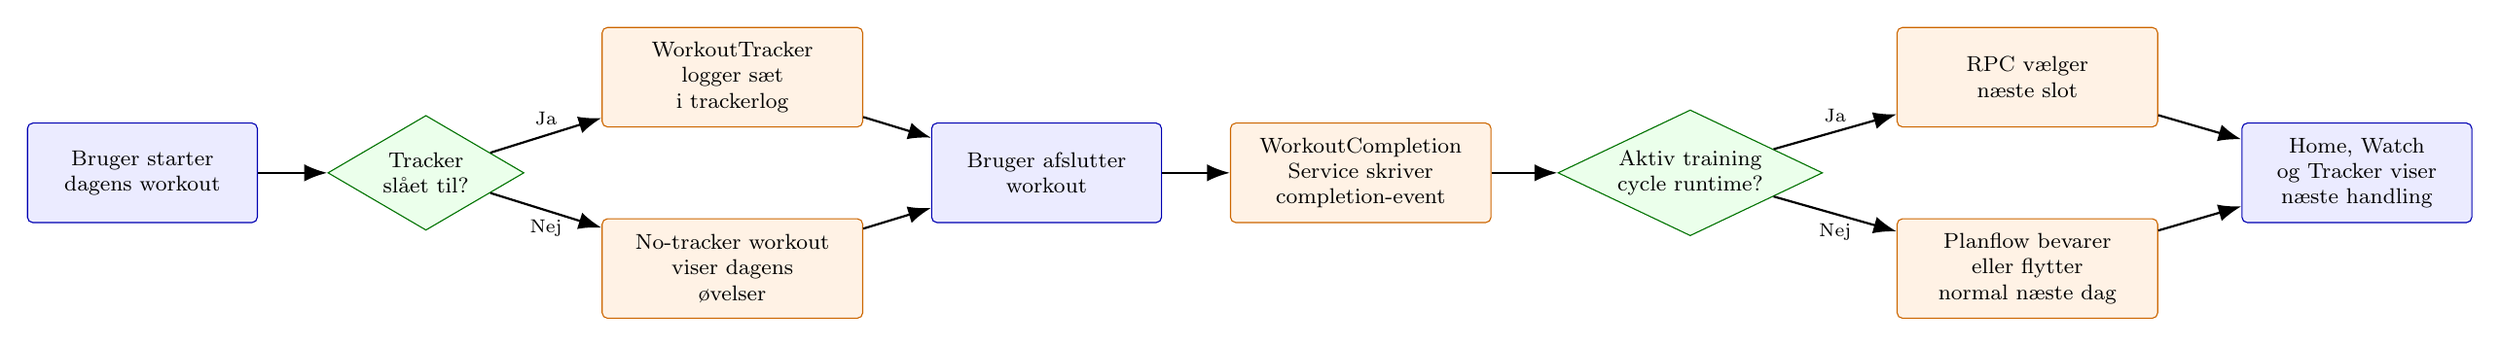
\begin{tikzpicture}[
    >={Latex[length=3mm]},
    node distance=12mm,
    tmuser/.style={draw=blue!70!black, fill=blue!8, rounded corners=2pt, align=center, minimum width=30mm, minimum height=13mm, font=\footnotesize},
    tmdata/.style={draw=orange!80!black, fill=orange!10, rounded corners=2pt, align=center, minimum width=34mm, minimum height=13mm, font=\footnotesize},
    tmdecision/.style={diamond, aspect=2.1, draw=green!45!black, fill=green!8, align=center, inner sep=1.5pt, minimum width=24mm, minimum height=15mm, font=\footnotesize},
    tmarrow/.style={->, line width=0.8pt}
]
\node[tmuser] (start) at (0,0) {Bruger starter\\dagens workout};
\node[tmdecision] (tracker) at (3.7,0) {Tracker\\slået til?};
\node[tmdata] (logging) at (7.7,1.25) {WorkoutTracker\\logger sæt\\i trackerlog};
\node[tmdata] (notracker) at (7.7,-1.25) {No-tracker workout\\viser dagens\\øvelser};
\node[tmuser] (finish) at (11.8,0) {Bruger afslutter\\workout};
\node[tmdata] (completion) at (15.9,0) {WorkoutCompletion\\Service skriver\\completion-event};
\node[tmdecision] (cycle) at (20.2,0) {Aktiv training\\cycle runtime?};
\node[tmdata] (rpc) at (24.6,1.25) {RPC vælger\\næste slot};
\node[tmdata] (planflow) at (24.6,-1.25) {Planflow bevarer\\eller flytter\\normal næste dag};
\node[tmuser] (next) at (28.9,0) {Home, Watch\\og Tracker viser\\næste handling};

\draw[tmarrow] (start) -- (tracker);
\draw[tmarrow] (tracker) -- node[above, font=\scriptsize] {Ja} (logging);
\draw[tmarrow] (tracker) -- node[below, font=\scriptsize] {Nej} (notracker);
\draw[tmarrow] (logging) -- (finish);
\draw[tmarrow] (notracker) -- (finish);
\draw[tmarrow] (finish) -- (completion);
\draw[tmarrow] (completion) -- (cycle);
\draw[tmarrow] (cycle) -- node[above, font=\scriptsize] {Ja} (rpc);
\draw[tmarrow] (cycle) -- node[below, font=\scriptsize] {Nej} (planflow);
\draw[tmarrow] (rpc) -- (next);
\draw[tmarrow] (planflow) -- (next);
\end{tikzpicture}%
}
\captionof{figure}{Opsummering af tracker-on/off, completion-event og progression i træningscyklus.}
\label{fig:tm-tracker-completion-summary}
\end{center}
\vspace*{\fill}
\end{landscape}
\clearpage
}

\subsection{App-screenshots}

\tmscreenshot{Materiale/traeningsmester-2026-04-28/02_figurer_og_screenshots/app_screenshots/aktuel_ios26/ios26-01-home-stale-session-testkonto-2026-04-28.jpg}{Home-skærm med advarsel om en forældet tracker-session og mulighed for at fortsætte eller rydde sessionen.}{fig:tm-ios-home-stale-session}

\tmscreenshot{Materiale/traeningsmester-2026-04-28/02_figurer_og_screenshots/app_screenshots/aktuel_ios26/ios26-02-home-ready-testkonto-2026-04-28.jpg}{Home-skærm med aktuel træningshandling og næste planlagte træningspas.}{fig:tm-ios-home-ready}

\tmscreenshot{Materiale/traeningsmester-2026-04-28/02_figurer_og_screenshots/app_screenshots/aktuel_ios26/ios26-03-programmer-testkonto-2026-04-28.jpg}{Programoversigt med aktiv programstruktur og brugerens valgte progression.}{fig:tm-ios-programmer}

\tmscreenshot{Materiale/traeningsmester-2026-04-28/02_figurer_og_screenshots/app_screenshots/aktuel_ios26/ios26-04-oevelser-testkonto-2026-04-28.jpg}{Øvelseskatalog med søgning, filtrering og øvelsesliste i den aktuelle iOS-version.}{fig:tm-ios-oevelser}

\tmscreenshot{Materiale/traeningsmester-2026-04-28/02_figurer_og_screenshots/app_screenshots/aktuel_ios26/ios26-05-match-card-testkonto-2026-04-28.jpg}{Match-flow med swipe-kort til inspiration og valg af øvelser.}{fig:tm-ios-match-card}

\tmscreenshot{Materiale/traeningsmester-2026-04-28/02_figurer_og_screenshots/app_screenshots/aktuel_ios26/ios26-06-indstillinger-testkonto-2026-04-28.jpg}{Indstillingsoversigt med kontosektion og brugerens aktuelle app-tilstande.}{fig:tm-ios-indstillinger}

\tmscreenshot{Materiale/traeningsmester-2026-04-28/02_figurer_og_screenshots/app_screenshots/aktuel_ios26/ios26-07-konto-loginmetoder-testkonto-2026-04-28.jpg}{Kontoens loginmetoder i indstillingsflowet.}{fig:tm-ios-konto-loginmetoder}

\tmscreenshot{Materiale/traeningsmester-2026-04-28/02_figurer_og_screenshots/app_screenshots/aktuel_ios26/ios26-08-premium-abonnement-testkonto-2026-04-28.jpg}{Premium- og abonnementsvisning med appens betalingsrelaterede funktionsadgang.}{fig:tm-ios-premium-abonnement}

\tmscreenshot{Materiale/traeningsmester-2026-04-28/02_figurer_og_screenshots/app_screenshots/aktuel_ios26/ios26-09-historik-testkonto-2026-04-28.jpg}{Historikvisning med tidligere træningslog og gennemførte pas.}{fig:tm-ios-historik}

\tmscreenshot{Materiale/traeningsmester-2026-04-28/02_figurer_og_screenshots/app_screenshots/aktuel_ios26/ios26-10-tracker-active-testkonto-2026-04-28.jpg}{Aktiv tracker-session med planlagte sæt og løbende registrering under træning.}{fig:tm-ios-tracker-active}

\tmscreenshot{Materiale/traeningsmester-2026-04-28/02_figurer_og_screenshots/app_screenshots/aktuel_ios26/ios26-11-home-completion-delay-testkonto-2026-04-28.jpg}{Home-skærm efter gennemført pas med forsinket completion-feedback og fortrydelsesvindue.}{fig:tm-ios-home-completion-delay}

\tmscreenshot{Materiale/traeningsmester-2026-04-28/02_figurer_og_screenshots/app_screenshots/aktuel_ios26/ios26-12-home-next-training-testkonto-2026-04-28.jpg}{Home-skærm efter completion, hvor næste træningshandling er rykket frem.}{fig:tm-ios-home-next-training}

\tmscreenshot{Materiale/traeningsmester-2026-04-28/02_figurer_og_screenshots/app_screenshots/aktuel_ios26/ios26-13-home-current-xcode-mcp-qa-2026-04-28.jpg}{Home-skærm efter gennemløb med Dagens træning synlig.}{fig:tm-ios-home-current-qa}

\tmlandscapediagramwithsection{Arkitektur- og dataflowdiagrammer}{assets/bilag/diagrammer/system_context.pdf}{0bp 532bp 0bp 0bp}{Systemkontekst for Træningsmester på iOS, watchOS, Supabase og Apple-services.}{fig:tm-system-context}

\tmlandscapewidediagram{assets/bilag/diagrammer/data_model_er.pdf}{0bp 610bp 0bp 0bp}{ER-diagram for programmer, workouts, tracker, completion, settings og cyklusdata.}{fig:tm-data-model-er}

\tmlandscapeerdetail{assets/bilag/diagrammer/data_model_er.pdf}{0bp 610bp 360bp 0bp}{ER-diagram, venstre udsnit: bruger, programmer, workouts og deling.}{fig:tm-data-model-er-left}

\tmlandscapeerdetail{assets/bilag/diagrammer/data_model_er.pdf}{180bp 610bp 180bp 0bp}{ER-diagram, midterudsnit: settings, workouts, øvelser, trackerlog og completion-events.}{fig:tm-data-model-er-middle}

\tmlandscapeerdetail{assets/bilag/diagrammer/data_model_er.pdf}{360bp 610bp 0bp 0bp}{ER-diagram, højre udsnit: træner-/klientrelationer og træningscyklusdata.}{fig:tm-data-model-er-right}

\tmtrackercompletiondiagram

\tmlandscapediagram{assets/bilag/diagrammer/security_boundary_summary.pdf}{0bp 590bp 0bp 0bp}{Sikkerhedsgrænse mellem mobil klient, RLS og Edge Functions.}{fig:tm-security-boundary-summary}

\tmlandscapediagram{assets/bilag/diagrammer/watch_sync_sequence.pdf}{10bp 610bp 10bp 0bp}{Sekvens for iOS/watchOS auth-sync, token-cache og RLS-baseret workoutdata.}{fig:tm-watch-sync-sequence}

\tmlandscapediagram{assets/bilag/diagrammer/live_activity_idempotency_sequence.pdf}{15bp 515bp 15bp 5bp}{Sekvens for Live Activity intent-write, App Group snapshot og idempotent trackerlog.}{fig:tm-live-activity-idempotency-sequence}

\tmlandscapediagram{assets/bilag/diagrammer/import_ai_edge_boundary.pdf}{0bp 585bp 0bp 0bp}{Import/AI-grænse mellem klient, Edge Functions, OpenAI og Supabase.}{fig:tm-import-ai-edge-boundary}

\subsection{Materialegennemgang}

\begin{table}[htbp]
\small
\renewcommand{\arraystretch}{1.18}
\begin{tabularx}{\textwidth}{>{\raggedright\arraybackslash}p{0.23\textwidth} >{\raggedright\arraybackslash}p{0.28\textwidth} Y}
\textbf{Bilagsspor} & \textbf{Faglig funktion} & \textbf{Begrundelse} \\
\hline
Aktuelle app-screenshots & Dokumenterer den aktuelle brugerflade & Figurerne \ref{fig:tm-ios-home-stale-session}--\ref{fig:tm-ios-home-current-qa} viser centrale flows i iOS 26.4-versionen af Træningsmester. \\
Arkitektur- og dataflowdiagrammer & Dokumenterer systemets tekniske hovedstruktur & Figurerne \ref{fig:tm-system-context}--\ref{fig:tm-import-ai-edge-boundary} dækker systemkontekst, datamodel med forstørrede ER-udsnit, tracker/completion, RLS, watchOS, Live Activity og import/AI-grænser. \\
Containerarkitektur & Samler arkitekturen i komponentlag & Tabel \ref{tab:tm-container-architecture} gør hovedlagene læsbare som tekstligt overblik. \\
Trackerproces og autorisationsregler & Forklarer træningsflow og sikkerhedsmodel & Tabel \ref{tab:tm-tracker-flow-bpmn} og \ref{tab:tm-authorization-dcr} viser de centrale proces- og adgangsregler. \\
Use cases og kravsporbarhed & Kobler funktionalitet til implementering og test & Tabel \ref{tab:tm-use-cases} og \ref{tab:tm-krav-traceability} viser sammenhængen mellem brugerhandlinger, krav og implementeringsspor. \\
SQL, RLS og sikkerhed & Dokumenterer data- og adgangsmodellen & Tabel \ref{tab:tm-sql-domain-overblik}, \ref{tab:tm-sql-fields} og \ref{tab:tm-rls-matrix} beskriver datadomæner, idempotency-felter og sikkerhedsgrænser. \\
Beta- og TestFlight-spor & Dokumenterer iteration og brugerindsigt & Tabel \ref{tab:tm-testflight-timeline} og \ref{tab:tm-beta-feedback} samler anonymiserede observationspunkter uden direkte citater eller persondata. \\
Afgrænset råmateriale & Understøtter anonymisering og versionsklarhed & Private rådata, lukkede kommunikationsspor og ældre UI-optagelser er fravalgt af hensyn til samtykke, dataminimering og klarhed om den dokumenterede appversion. \\
\end{tabularx}
\caption{Gennemgang af bilagsmateriale og afgrænsning.}
\label{tab:tm-bilag-materialegennemgang}
\end{table}

\clearpage

\subsection{Use cases og krav}

\begin{table}[htbp]
\footnotesize
\renewcommand{\arraystretch}{1.12}
\begin{tabularx}{\textwidth}{>{\raggedright\arraybackslash}p{0.17\textwidth} >{\raggedright\arraybackslash}p{0.30\textwidth} Y}
\textbf{Use case} & \textbf{Kort formål} & \textbf{Faglig relevans} \\
\hline
UC-01 Opret konto og log ind & Supabase Auth, session restore og app-shell efter autentifikation. & Viser auth som forudsætning for brugerbundne træningsdata og RLS. \\
UC-02 Gennemfør onboarding & Valg af startvej, præferencer og eventuel programimport. & Understøtter analyse af første brugerrejse og friktion. \\
UC-03 Opret/rediger program & Oprette, hente, opdatere, aktivere og dele træningsprogrammer. & Dokumenterer programstruktur som kernefunktion. \\
UC-04 Tilføj træningsdag og øvelser & Knytte workouts og øvelser til programmet med sæt, reps, vægt og pause. & Knytter planlægning til den konkrete træningsfaglige struktur. \\
UC-05 Find og like øvelse & Søge, swipe og gemme liked/parrede øvelser. & Kobler øvelseskatalog, søgning og match-flow til brugerfeedback. \\
UC-06 Start workout med tracker & Logge sæt, styre pauser, opdatere Live Activity og gemme completion. & Central use case for fleksibel progression og lav-friktionslogging. \\
UC-07 Brug watchOS companion & Vise dagens træning og logge/afslutte workout fra Apple Watch. & Dokumenterer multiplatform-sporet uden runtime-screenshots. \\
UC-08 Aktiv træningscyklus & Prioritere cyklus-runtime over lineær planindekslogik. & Underbygger progression, deload og afvigelseshåndtering. \\
UC-09 Træner administrerer klient & Træner ser klienter, aktivitet og programlinks via servervalideret relation. & Afgrænser trænerfunktioner som teknisk udvidelse, ikke hovedproblem. \\
UC-10 Admin håndterer bruger eller aktivitet & Admin-center gennem Edge Function og server-side admin guard. & Underbygger governance, katalogkvalitet og sikkerhedsdesign. \\
UC-11 Importer program eller historik & Importjob, normalisering, preview og gem af program/historikkladder. & Viser AI/import som afgrænset server-side flow. \\
\end{tabularx}
\caption{Kondenseret use case-overblik for Træningsmester.}
\label{tab:tm-use-cases}
\end{table}

\begin{table}[htbp]
\footnotesize
\renewcommand{\arraystretch}{1.12}
\begin{tabularx}{\textwidth}{>{\raggedright\arraybackslash}p{0.23\textwidth} >{\raggedright\arraybackslash}p{0.19\textwidth} Y}
\textbf{Use case} & \textbf{Dækkede krav} & \textbf{Primære implementeringsspor} \\
\hline
UC-01 Opret konto og log ind & F-01, F-02, NF-01, NF-02 & Login, AppState, AppEnvironment, Supabase repositories. \\
UC-02 Gennemfør onboarding & F-02, F-11, F-12 & Onboardingmodeller, onboarding-flow og ProgramReviewService. \\
UC-03 Opret/rediger træningsprogram & F-03, F-04, NF-02, NF-03 & TrainingProgramView, AddProgramView og PlanRepository. \\
UC-04 Tilføj træningsdag og øvelser & F-04, F-05, F-06 & WorkoutRepository, TrackerRepository og workout exercise payloads. \\
UC-05 Find og like øvelse & F-06, F-07 & ExercisesView, MatchView og ExerciseSearchCatalog. \\
UC-06 Start workout med tracker & F-08, F-09, F-10, F-15 & WorkoutTrackerView, WorkoutCompletionService og Live Activity-spor. \\
UC-07 Brug watchOS companion & F-14, F-08, F-09, NF-07 & WatchWorkoutStore og WatchAuthSyncBridge. \\
UC-08 Aktiv træningscyklus & F-13, F-08, F-14 & TrainingCycleViews, TrainingCycleRepository og cycle RPC. \\
UC-09 Træner administrerer klient & F-16, NF-02, NF-08 & ClientsView, TrainerClientService og trainer-client Edge Function. \\
UC-10 Admin håndterer bruger & F-17, NF-01, NF-02 & SettingsView, admin-control-center og admin SQL functions. \\
UC-11 Importer program/historik & F-12, NF-08 & PremiumView, ProgramReviewService og import Edge Functions. \\
\end{tabularx}
\caption{Sporbarhed mellem use cases, krav og implementeringsspor.}
\label{tab:tm-krav-traceability}
\end{table}

\clearpage

\subsection{Arkitektur-, proces- og autorisationsmodeller}

\begin{table}[htbp]
\small
\renewcommand{\arraystretch}{1.15}
\begin{tabularx}{\textwidth}{>{\raggedright\arraybackslash}p{0.22\textwidth} >{\raggedright\arraybackslash}p{0.36\textwidth} Y}
\textbf{Lag} & \textbf{Indhold} & \textbf{Faglig brug} \\
\hline
iOS-app & SwiftUI-features, RootView, AppState, domain models, repository protocols, Supabase repositories, support services og designsystem. & Viser at UI, state og dataadgang er opdelt i lag frem for direkte databasekald fra views. \\
watchOS-app & WatchRootView, WatchWorkoutStore og WatchAuthSyncBridge. & Dokumenterer watchOS som companion til dagens træning og hurtig logging. \\
Extensions & Live Activity widget, Live Activity intents og watch widget/complication. & Underbygger lav-friktionsstatus under træning uden fuld appåbning. \\
Supabase & Auth, Postgres med RLS/views/RPC og Storage. & Viser backendens rolle som auth-, data- og sikkerhedsgrænse. \\
Edge Functions & Admin, trainer-client, program/import/analyse og billing functions. & Afgrænser privilegerede operationer til server-side runtime. \\
Apple services & StoreKit 2, WatchConnectivity, ActivityKit/WidgetKit og HealthKit. & Placering af platformservices og afgrænsning af integrationer. \\
\end{tabularx}
\caption{Komponentoverblik for Træningsmesters arkitektur.}
\label{tab:tm-container-architecture}
\end{table}

\begin{table}[htbp]
\small
\renewcommand{\arraystretch}{1.15}
\begin{tabularx}{\textwidth}{>{\raggedright\arraybackslash}p{0.24\textwidth} >{\raggedright\arraybackslash}p{0.34\textwidth} Y}
\textbf{Procespunkt} & \textbf{Kondenseret procesindhold} & \textbf{Faglig brug} \\
\hline
Start og session & Brugeren starter workout; AppState validerer auth og profile mode. & Viser at træningsflowet er brugerbundet og sessionafhængigt. \\
Tracker-valg & Gateway afgør, om tracker er aktiveret. & Gør tracker-off completion til en legitim vej gennem flowet. \\
Tracker-route & Appen åbner workoutTracker, henter øvelser og historik og synkroniserer Live Activity snapshot. & Dokumenterer sammenhæng mellem planlagt workout, faktisk logging og statusflade. \\
No-tracker-route & Appen åbner workoutTrackerWithoutLogging og går direkte mod completion. & Understøtter håndtering af afvigelser uden tvungen sætlogning. \\
Log-sæt-loop & Brugeren indtaster reps, vægt eller varighed; repository skriver trackerlog og opdaterer projection. & Viser hvordan gentagne sæt håndteres i et loop. \\
Completion & WorkoutCompletionService gemmer completion event. & Adskiller gennemført træning fra detaljeret trackerlog. \\
Progression & Aktiv cyklus kalder progression RPC efter completion. & Kobler completion til næste træningshandling og cyklusprogression. \\
Historik/Home & Historik og Home bruger completion- og trackerlogdata efter afslutning. & Viser feedback tilbage til brugerens næste app-state. \\
\end{tabularx}
\caption{Tracker- og completionproces for Træningsmester.}
\label{tab:tm-tracker-flow-bpmn}
\end{table}

\begin{table}[htbp]
\small
\renewcommand{\arraystretch}{1.15}
\begin{tabularx}{\textwidth}{>{\raggedright\arraybackslash}p{0.22\textwidth} >{\raggedright\arraybackslash}p{0.40\textwidth} Y}
\textbf{Autorisationsspor} & \textbf{Kondenseret regel} & \textbf{Faglig brug} \\
\hline
Miljø og klient & Appen loader miljø, afviser placeholder- eller service-role keys og opretter derefter anon Supabase client. & Underbygger beslutningen om, at service-role ikke må ligge i klienten. \\
Session og brugerdata & AuthenticateUser og ResolveSession er forudsætning for ReadOwnData, WriteOwnData og delt planadgang. & Viser auth som betingelse for brugerbundne læse-/skrivehandlinger. \\
Admin & CallAdminFunction kræver ResolveSession; derefter skal ValidateAdminServerSide ske, ellers afvises operationen. & Dokumenterer at admin-UI ikke er autoritativt i sig selv. \\
Trainer/import & Service-role er kun legal inside Edge Function runtime for trainer-, admin- eller importfunktioner. & Afgrænser privilegeret adgang til backend. \\
Tracker og Live Activity & WriteTrackerLog kræver session; Live Activity write kræver session og deduplicering via client action. & Understøtter idempotency og RLS i træningslogging. \\
Afvisning og audit & Cross-user access afvises, og privilegerede mutationer bør persistere audit event. & Kobler sikkerhed, governance og sporbarhed. \\
\end{tabularx}
\caption{Autorisationsregler for Træningsmester.}
\label{tab:tm-authorization-dcr}
\end{table}

\clearpage

\subsection{SQL, RLS og sikkerhed}

\begin{table}[htbp]
\small
\renewcommand{\arraystretch}{1.15}
\begin{tabularx}{\textwidth}{>{\raggedright\arraybackslash}p{0.22\textwidth} >{\raggedright\arraybackslash}p{0.36\textwidth} Y}
\textbf{Domæne} & \textbf{Centrale tabeller} & \textbf{Formål} \\
\hline
Øvelseskatalog & exercises, workout exercise user weights & Officielle/private øvelser, søgning, medier og brugerspecifik vægt. \\
Programmer & plan, workout, plan workouts, workout exercises & Programstruktur, træningsdage og øvelsesrækker. \\
Deling/social & plan share codes, shared users, invites, friend codes og friendships & Programdeling, invites og buddy-relationer. \\
Træner/klient & trainer clients og trainer client plan links & Klientrelationer og planadgang. \\
Match & match og liked/parrede views & Like-/swipe-state for øvelser. \\
Tracker/historik & trackerlog, workout completion events og active workout session state & Sætlogs, completion uden trackerlog og aktiv session. \\
Settings/admin & user settings, activity events, feedback, version history og error reports & Profiltilstand, subscription, admin, feedback og diagnostics. \\
Cykler/import & training cycles, cycle runtime-tabeller og training import jobs & Makro/meso/deload, runtime progression og importjobs. \\
\end{tabularx}
\caption{Centrale SQL-domæner i Træningsmesters datamodel.}
\label{tab:tm-sql-domain-overblik}
\end{table}

\begin{table}[htbp]
\small
\renewcommand{\arraystretch}{1.15}
\begin{tabularx}{\textwidth}{>{\raggedright\arraybackslash}p{0.24\textwidth} >{\raggedright\arraybackslash}p{0.24\textwidth} Y}
\textbf{Felt} & \textbf{Placering} & \textbf{Hvorfor feltet er relevant} \\
\hline
profile mode & User settings, completion, session og cycle flows & Skelner personlig bruger fra træner-/klientkontekst. \\
client action id & Trackerlog og workout completion events & Giver idempotency for Live Activity-, watch- og tracker-writes. \\
reverted at & Workout completion events & Gør det muligt at fortryde completion uden at slette historik. \\
superset group og position & Workout exercises & Understøtter superset-struktur i tracker og watch. \\
rest override & Workout exercises & Skelner standardpause fra bevidst pauseoverride. \\
subscription tier & User settings & Binder StoreKit-køb til appens featureadgang. \\
is admin & User settings & Bruges sammen med servervalidering, ikke som eneste adminbevis. \\
\end{tabularx}
\caption{Særligt relevante SQL-felter i Træningsmesters datamodel.}
\label{tab:tm-sql-fields}
\end{table}

\begin{table}[htbp]
\footnotesize
\renewcommand{\arraystretch}{1.12}
\begin{tabularx}{\textwidth}{>{\raggedright\arraybackslash}p{0.19\textwidth} >{\raggedright\arraybackslash}p{0.25\textwidth} >{\raggedright\arraybackslash}p{0.25\textwidth} Y}
\textbf{Område} & \textbf{Primær sikkerhedsgrænse} & \textbf{Klientbeskyttelse} & \textbf{Server/SQL-beskyttelse} \\
\hline
Auth/session & Supabase Auth og anon key & AppEnvironment afviser placeholders/service-role. & Auth JWT og auth.uid(). \\
Egne programmer & RLS på plan/workout-tabeller & Repositories kræver session og typed payloads. & Owner policies og helper functions. \\
Delte programmer & RLS og share views & UI viser kun accessible resources. & Read/edit helpers for delt planadgang. \\
Trackerlog & RLS og immutable field trigger & Tracker repositories sender brugerbundne writes. & Immutable trigger og unik client action. \\
Completion events & RLS og idempotency & Completion-service centraliserer skrivninger. & Unik user/action og reverted-at-felt. \\
Active session & RLS og forced RLS & App state og Live Activity snapshot. & Unique user/profile session og constraints. \\
Watch sync & App Group/local cache og anon session & Watch token payload model. & RLS for backend reads/writes. \\
Live Activity intents & App Group snapshot og anon Supabase client & SharedStore og projectionmodel. & RLS og idempotente writes. \\
Admin & Edge Function og SQL guard & UI viser kun adminflow efter server-backed state. & Admin guards og service-role kun i function runtime. \\
Trainer/client & Edge Function og RLS & Trainer-client-service. & Related-user policies og trainer-client function. \\
AI/import & Edge Functions & Klienten kalder ikke OpenAI direkte. & Function runtime styrer service-role/OpenAI. \\
\end{tabularx}
\caption{RLS- og sikkerhedsmatrix for Træningsmester.}
\label{tab:tm-rls-matrix}
\end{table}

\clearpage

\subsection{Beta, brugerindsigt og verifikation}

\begin{table}[htbp]
\footnotesize
\renewcommand{\arraystretch}{1.08}
\begin{tabularx}{\textwidth}{>{\raggedright\arraybackslash}p{0.18\textwidth} >{\raggedright\arraybackslash}p{0.16\textwidth} >{\raggedright\arraybackslash}p{0.18\textwidth} Y}
\textbf{Dato} & \textbf{Version/build} & \textbf{Platform} & \textbf{Faglig brug} \\
\hline
2026-03-25 22:20 UTC & Invitation & iOS & Start på iOS-beta og formel rekruttering. \\
2026-03-26 16:29 UTC & 1.0 (5) & iOS + watchOS & Første observerede build efter invitation. \\
2026-03-27 13:02 UTC & 1.0 (6) & iOS + watchOS & Iteration samme uge som betaåbning. \\
2026-03-27 13:17 UTC & 1.0 (8) & iOS + watchOS & Hurtig efterfølgende build. \\
2026-03-29 23:29 UTC & 2.0 (1) & iOS + watchOS & Skift til 2.0-sporet. \\
2026-03-30 23:07 UTC & 2.0 (2) & iOS + watchOS & Build omkring link-/opdateringsfriktion. \\
2026-03-31 00:09 UTC & 2.0 (3) & iOS + watchOS & Natlig iteration op til større releasebesked. \\
2026-03-31 10:58 UTC & 2.0 (4) & iOS + watchOS & Samme dag som katalog-, søgnings- og releasefeedback. \\
2026-03-31 19:24 UTC & 2.0 (5) & iOS + watchOS & Iterativ build efter feedback samme dag. \\
2026-04-01 18:19 UTC & 2.0 (6) & iOS + watchOS & Fortsat testdistribution efter martsfeedback. \\
2026-04-15 00:40 UTC & 2.0 (7) & iOS + watchOS & Ny beta efter april-iteration. \\
2026-04-15 01:02 UTC & 2.0 (8) & iOS + watchOS & Hurtig efterfølgende iteration. \\
2026-04-20 00:57 UTC & 2.0 (9) & iOS + watchOS & Pre-audit/releasekandidat. \\
2026-04-23 15:19 UTC & 2.0 (10) & iOS + watchOS & Sen beta med fortsat polish. \\
2026-04-23 23:37 UTC & 2.0 (11) & iOS + watchOS & Samme døgn som build 10; kort releasecyklus. \\
2026-04-25 21:01 UTC & 2.0 (12) & iOS + watchOS & Seneste observerede beta-build i den gennemgåede betaperiode. \\
\end{tabularx}
\caption{TestFlight-tidslinje for Træningsmester. Tabellen dokumenterer distribution og iteration, ikke sundhedseffekt.}
\label{tab:tm-testflight-timeline}
\end{table}

\begin{table}[htbp]
\footnotesize
\renewcommand{\arraystretch}{1.12}
\begin{tabularx}{\textwidth}{>{\raggedright\arraybackslash}p{0.14\textwidth} >{\raggedright\arraybackslash}p{0.18\textwidth} >{\raggedright\arraybackslash}p{0.32\textwidth} Y}
\textbf{ID} & \textbf{Tema} & \textbf{Anonymiseret observation} & \textbf{Designimplikation} \\
\hline
B01 & Friktion & Lock screen/Live Activity blev bekræftet som fungerende i praktisk brug. & Prioriter hurtig status under træning uden fuld appåbning. \\
B02 & Mediekvalitet & Dialogen pegede på ønske om rigtige øvelsesvideoer frem for generiske klip. & Øvelsesmedier skal være troværdige og kropsligt genkendelige. \\
B05 & Betaproces & Build 4-12 blev distribueret mellem 2026-03-31 og 2026-04-25. & Dokumenterer iterationstempo, men ikke brugerudbytte alene. \\
B10 & Rekruttering & iOS-kravet udelukkede mindst én interesseret deltager. & Betaen bør beskrives som iOS-biased convenience sample. \\
B11 & Installationsfriktion & TestFlight-link, Apple review-status og manuel opdatering skabte forvirring. & Beta-onboarding skal vise build/version og fallback-instruktion tydeligt. \\
B12 & Katalog & Risiko for dubletter og lav datakvalitet ved fri øvelsesoprettelse. & Private øvelser og offentligt katalog bør adskilles med review-flow. \\
B13 & Søgning & Tester kunne ikke finde almindelige øvelser eller varianter i betaen. & Søgning skal understøtte synonymer, varianter og øvelsesfamilier. \\
B15 & Enheder & Tester ønskede kg/lbs, fordi nogle maskiner bruger lbs. & Tilbyd global enhed, per-øvelse override og logkonvertering. \\
B16 & Watch & Apple Watch blev positioneret som telefonfri træningsflade med stabilitetsforbehold. & Prioriter oversigt, hurtig logging og robust session-sync. \\
B18 & Noter & Feedback pegede på behov for noter til teknik, udstyr eller sædeindstilling. & Øvelsesnoter bør behandles som træningskontekst, ikke kun fritekst. \\
\end{tabularx}
\caption{Udvalgte anonymiserede betaobservationer. Direkte citater og personhenførbare detaljer er fravalgt.}
\label{tab:tm-beta-feedback}
\end{table}

\begin{table}[htbp]
\small
\renewcommand{\arraystretch}{1.15}
\begin{tabularx}{\textwidth}{>{\raggedright\arraybackslash}p{0.26\textwidth} >{\raggedright\arraybackslash}p{0.25\textwidth} Y}
\textbf{Teknisk påstand} & \textbf{Dokumenteret status} & \textbf{Begrænsning} \\
\hline
Appen kan bygges som iOS-klient & Bestået & Ikke dokumenteret som uafhængig reproducerbar build. \\
Central forretningslogik er unit-testet & Bestået & Dækker unit-lag, ikke alle live backendscenarier. \\
Supabase anon read path fungerer & Delvist bestået & Tests med admin- og ikke-admin-legitimationsoplysninger blev sprunget over. \\
watchOS targetet kan bygges & Bestået & Runtime-forløb er ikke dokumenteret visuelt i bilaget. \\
Live Activity targetet kan bygges & Bestået & Dynamic Island-forløb er ikke dokumenteret visuelt i bilaget. \\
Aktuel iOS UI er dokumenteret visuelt & Bestået & Bygger på de aktuelle screenshots, der er indsat i bilaget. \\
Data-/sikkerhedsmodellen er dokumenteret & Stærk dokumentation & Fuld security proof kræver flere integrationstests. \\
\end{tabularx}
\caption{Verifikationsspor for tekniske claims.}
\label{tab:tm-test-traceability}
\end{table}

\clearpage
\fussy


\end{document}
